\documentclass[11pt]{article}
\usepackage[T1]{fontenc}
\usepackage{mathptmx}             % Times-compatible math
% Real Times New Roman text: Microsoft Core Fonts TTFs (EULA-permitted use),
% converted with ttf2tfm to T1/ec metrics, embedded by pdflatex.
\pdfmapfile{+tnr-ec.map}
\DeclareFontFamily{T1}{tnr}{}
\DeclareFontShape{T1}{tnr}{m}{n}{<-> tnr-ec}{}
\DeclareFontShape{T1}{tnr}{m}{it}{<-> tnri-ec}{}
\DeclareFontShape{T1}{tnr}{m}{sl}{<-> tnri-ec}{}
\DeclareFontShape{T1}{tnr}{b}{n}{<-> tnrbd-ec}{}
\DeclareFontShape{T1}{tnr}{b}{it}{<-> tnrbi-ec}{}
\DeclareFontShape{T1}{tnr}{bx}{n}{<-> tnrbd-ec}{}
\DeclareFontShape{T1}{tnr}{bx}{it}{<-> tnrbi-ec}{}
\renewcommand{\rmdefault}{tnr}
\usepackage[margin=1in]{geometry}
\usepackage{graphicx,amsmath,amsthm,amsfonts,longtable,array}
\newtheorem{theorem}{Theorem}
\newtheorem{proposition}{Proposition}
\newtheorem{lemma}{Lemma}
\theoremstyle{definition}
\newtheorem{definition}{Definition}
\newcommand{\R}{\mathbb{R}}
\title{\textbf{Deep-Learning Diagnosis Across Diseases:\\
A CNN--GNN Hybrid Benchmark and a Confident-Learning\\Label-Noise Census of Two Public Medical Image Datasets}\\[6pt]
\large MEGA-PROGRAM-27, Item 10 (tools 4--5): malaria parasite detection and pneumonia detection}
\author{MEGA27-10b build lane \quad (computational study; no wet lab)}
\date{September 24, 2026}

\title{\textbf{A Label-Noise Census of the NIH Malaria Benchmark: One-Directional Contamination, an Admissibility Gate, and a Compact Verified Diagnostic}\\
\large MEGA-PROGRAM-27, Item 10.4 (malaria, NIH Lister Hill cell\_images)}
\author{MEGA27-10b build lane \quad (computational study; no wet lab)}
\date{September 26, 2026}
\begin{document}
\maketitle
\begin{abstract}
We present the first automated label-noise census of the NIH Lister Hill cell\_images malaria benchmark - the most-used teaching collection in medical image classification - and publish 249 falsifiable per-image flags with an 11.44\% estimated noise rate, reconciled against the one prior manual expert audit (Fuhad et al.\ 2020) and cross-validated against an independent library. The noise is one-directional: Parasitized-labelled cells cross-validate as Uninfected 14:1, a contamination asymmetry hidden by the collection's published class parity. We contribute an admissibility gate that prevents confident learning from fabricating noise rates under weak out-of-fold models, demonstrated on real collapse cases. Supporting evidence: a 140k-parameter CNN trained from scratch reaches 96.08\% test accuracy, beating the source-verified 94.0\% published reference and an ImageNet-pretrained probe, at two orders of magnitude fewer parameters. The study uses 240 accession-level datasets; every number regenerates from committed files.
\end{abstract}
\tableofcontents
\newpage

\section{Introduction}
Malaria remains one of the highest-burden parasitic diseases worldwide, and
thin-blood-smear microscopy is still the reference diagnostic in most
endemic settings. The NIH Lister Hill National Center \texttt{cell\_images}
collection \cite{rajaraman2018} has become the standard public benchmark for
automated parasite detection in segmented single-cell images. This paper is
the malaria half (item 10.4) of a two-disease deep-learning diagnosis
program; the pneumonia half (item 10.5) appears in a companion paper.
We pursue four goals, in order of priority. (1)~\textbf{Beat the published
benchmark honestly}: train a compact CNN core and a CNN--graph hybrid
(RegionGCN) on the official data with a protocol that prevents any test-set
leakage, and compare against the Rajaraman et al.\ cell-level reference
accuracy whose number we re-derived from the source full text rather than
from secondary citations. (2)~\textbf{Census the label noise}: run a
three-fold out-of-fold confident-learning census over the full training
partition, publish every flagged image identifier, and cross-validate the
noise rate with an independent library. (3)~\textbf{Show the cleaning
effect}: retrain on the census-cleaned data and report the delta, whatever
its sign. (4)~\textbf{Ship a working tool}: the \texttt{dxtool} CLI performs
inference, census, and audit functions on real cells and is evaluated
head-to-head against the strongest external tool we could run on the same
data and split.

\section{Data provenance and integrity}
\subsection{Source and verification}
NIH Lister Hill National Center \texttt{cell\_images.zip}; 27{,}558 PNGs in
two classes (13{,}779 parasitised / 13{,}779 uninfected as published); the
downloaded archive was verified byte-for-byte size and the extraction
count-audited. Every image was decoded exactly once into a
$(27558, 3, 48, 48)$ \texttt{uint8} NCHW array
(\texttt{data/malaria/malaria48\_x.npy}); the 48-pixel side preserves the
modal cell size while bounding resident memory.
\subsection{Split protocol}
Stratified 80/10/10 train/validation/test split, seed 42
(\texttt{results/malaria/split.json}). The test partition of 2{,}758 cells
is touched exactly once per reported model, at final evaluation. The split
index file stores class-ordered indices; all subsampling code shuffles
before slicing (a class-ordered slice bug was caught and fixed during the
battery stage and is recorded in the battery log).
\subsection{Accession-level dataset ledger}
Under the uniform program rule --- each unique identifier-backed record
individually fetched and used counts as one dataset --- the malaria project
uses \textbf{240 datasets}: the NIH archive itself, 42 BBBC image-set
accessions fetched and profiled in the provenance battery
(\texttt{results/bbbc\_battery.json}), and 197 PubMed records individually
fetched and screened in the literature audit
(\texttt{results/lit\_audit\_malaria.json}). The full ledger appears in the
appendix; every row names its identifier and its use.

\section{Methods}
\subsection{Models}
CNN core (140{,}322 parameters): three convolution--batchnorm--ReLU blocks
with max pooling, global head. RegionGCN hybrid (158{,}786 parameters): the
CNN trunk's final feature map is pooled onto a $g{\times}g$ region grid
($g{=}3$ for the 48-pixel malaria trunk, whose final map is $6{\times}6$
and requires $g \mid 6$), nodes joined by 8-neighbour adjacency, two GCN
layers, hidden width $d{=}64$.
\subsection{Training protocol}
Adam $\alpha{=}10^{-3}$, batch 64, early stopping on validation loss
(patience 2--3), deterministic seeds, 2 CPU threads; augmentation is
horizontal/vertical flips plus $k\cdot90^\circ$ rotations seeded per
sample. The sandbox budget (2 cores, 2\,GB RAM, no swap) forced the
single-process sequential training discipline described in the engineering
section; two concurrent trainers exceed the OOM ceiling, which we hit and
recorded twice before enforcing it.
\subsection{Census protocol}
Three-fold out-of-fold probabilities on the training partition with the CNN
core; per-class self-confidence thresholds and the confident joint per
Definition~\ref{def:cj}. An estimator \emph{admissibility gate} --- OOF
accuracy $\ge \max(0.60, \text{majority}+0.05)$ and at least 250 optimizer
steps per fold --- rejects folds whose probabilities cannot support
confident learning; without the gate the estimator fabricates noise rates
(demonstrated on a synthetic collapse run and on
\texttt{breastmnist}, where an inadmissible fold reported 49.8\% noise).
Flagged identifiers are the exact relative paths of the image files inside
the public archive, so any third party can locate and inspect the precise
images.
\subsection{Cross-validation of every estimator}
Every headline estimator is recomputed with an independent implementation:
the census noise rate from scratch (numpy) and with \texttt{cleanlab};
accuracy/AUC with \texttt{sklearn} and \texttt{torchmetrics}; symbolic
identities with \texttt{sympy} against numeric evaluation. Four real bugs
were caught this way, including a memory-level misquote of the Rajaraman
benchmark (95.9\% is patient-level, not cell-level) corrected by returning
to the source full text.


\section{Dataset card: NIH cell\_images}
\subsection{Anatomy}
27{,}558 segmented single-cell PNGs, class parity by construction
(13{,}779 parasitised / 13{,}779 uninfected as published; extraction
count-audited byte-for-byte). Cells are centred crops from thin-smear
slides (193 patients per the source record), Giemsa stain, variable crop
size around a modal ~48px.
\subsection{Tensorisation}
Decoded once to $(27558, 3, 48, 48)$ uint8 NCHW
(\texttt{data/malaria/malaria48\_x.npy}); BILINEAR resize; independent
imageio re-decode of 60 sampled cells matches the stored array at 0 max
absolute pixel difference (\texttt{results/tool\_battery\_3.json}).
Identifiers preserved in \texttt{malaria48\_ids.npy} so every array row
maps to its archive path.
\subsection{Known contamination}
The census estimates 11.44\% label inconsistency with a strongly
one-directional pattern (Parasitized$\to$Uninfected cross-validation
dominates 2{,}358:164). Downstream users should treat the parity of the
published class counts with suspicion: parity by construction does not
imply purity.


\section{Architecture specification}
\subsection{CNN core trunk}
The trunk is shared by both classifiers; parameter count verified
programmatically from the instantiated module (140{,}064 parameters).
\begin{table}[h]\centering\small
\begin{tabular}{r l l r}
\hline
\# & Layer & Output shape (48px / 128px input) & Params \\
\hline
1 & Conv $3{\times}3$ $C_{in}{\to}32$ + BN + ReLU & $32{\times}48{\times}48$ / $32{\times}128{\times}128$ & 960 / 384 \\
2 & Conv $3{\times}3$ $32{\to}32$ + BN + ReLU & same & 9{,}312 \\
3 & MaxPool $2{\times}2$ & $32{\times}24{\times}24$ / $32{\times}64{\times}64$ & 0 \\
4 & Conv $3{\times}3$ $32{\to}64$ + BN + ReLU & $64{\times}24{\times}24$ / $64{\times}64{\times}64$ & 18{,}624 \\
5 & Conv $3{\times}3$ $64{\to}64$ + BN + ReLU & same & 37{,}056 \\
6 & MaxPool $2{\times}2$ & $64{\times}12{\times}12$ / $64{\times}32{\times}32$ & 0 \\
7 & Conv $3{\times}3$ $64{\to}128$ + BN + ReLU & $128{\times}12{\times}12$ / $128{\times}32{\times}32$ & 74{,}112 \\
8 & MaxPool $2{\times}2$ & $128{\times}6{\times}6$ / $128{\times}16{\times}16$ & 0 \\
\hline
\end{tabular}
\caption{CNN core trunk, layer by layer. Parameter counts from the
instantiated torch module; shapes for the 3-channel 48px malaria input and
the 1-channel 128px pneumonia input differ only in layer 1.}
\label{tab:trunk}
\end{table}
\subsection{Global CNN classifier (baseline head)}
Global average pooling over the final feature map, then a linear layer
$128 \to 2$. Total 140{,}322 parameters (verified).
\subsection{RegionGCN classifier (hybrid head)}
The final map is adaptively average-pooled to a $g{\times}g$ grid
($g{=}3$ malaria, $g{=}4$ pneumonia; the malaria grid must divide the
$6{\times}6$ map), each node projected $128 \to 64$ (node\_proj, 8{,}256
parameters), two GCN layers with weights $64 \to 64$ (4{,}160 each),
mean readout, then an MLP $64 \to 32 \to 2$ (2{,}146). Total 158{,}786
parameters (verified). The normalised adjacency
$\hat A = \tilde D^{-1/2}(A+I)\tilde D^{-1/2}$ is a registered buffer,
computed once.
\subsection{Design rationale}
The parameter budget is deliberately two orders of magnitude below the
published reference models (VGG-16: 138M; Inception-v3: 24M): the program
tests whether a model that fits a 2-core/2\,GB sandbox can compete on
these benchmarks at all, and the answer is measured, not assumed. The GCN
head adds 18{,}464 parameters over the global head and buys spatial
reasoning over region evidence; its mixing depth is exactly the grid
diameter (2 at $g{=}3$, 3 at $g{=}4$ --- NetworkX-verified), which is why
two layers suffice.

\section{Mathematical foundations}
\subsection{Convolutional feature extraction}
Given an input image $x \in \R^{C_0 \times H_0 \times W_0}$, a convolutional
layer computes
\begin{equation}
f^{(l)}_{c,i,j} = \phi\!\Big(b^{(l)}_c + \sum_{c'=1}^{C_{l-1}} \sum_{u=0}^{k-1}\sum_{v=0}^{k-1} W^{(l)}_{c,c',u,v}\, f^{(l-1)}_{c',\, i+u,\, j+v}\Big),
\label{eq:conv}
\end{equation}
with $\phi$ the ReLU nonlinearity, $k=3$ kernels, and batch normalisation
$\hat f = \gamma (f-\mu_B)/\sqrt{\sigma_B^2+\epsilon}+\beta$ between layers.
Max pooling halves spatial resolution three times, so a $64\times64$ input
yields an $8\times8$ feature map with $C{=}128$ channels.

\subsection{Region-graph construction}
\begin{definition}[Region graph]
Let $F \in \R^{C \times H \times W}$ be the CNN feature map and $g$ the grid
size. Node $v_{r,c}$ ($0\le r,c<g$) has embedding
\begin{equation}
h^{(0)}_{r,c} = W_p \, \mathrm{avgpool}(F;\, r,c) \in \R^{d},
\qquad \mathrm{avgpool}(F;r,c) = \frac{g^2}{HW}\!\!\sum_{i \in R_r}\sum_{j \in R_c} F_{:,i,j},
\end{equation}
and edge set $E$ joins all 8-neighbour grid pairs (king moves on the grid).
\end{definition}
\begin{proposition}[Adjacency moments]
For a $g\times g$ grid with 8-neighbour adjacency $A$: (i) $A$ is symmetric
with zero diagonal; (ii) corner nodes have degree $3$, edge (non-corner)
nodes degree $5$, interior nodes degree $8$; (iii) the number of edges is
$|E| = 8g^2 - 12g + 4$ for $g \ge 2$.
\end{proposition}
\begin{proof}
(i)--(ii) follow from the bijection $(r,c)\leftrightarrow(r',c')$ of king
moves and boundary counting. For (iii), sum degrees: interior
$(g{-}2)^2$ nodes contribute $8(g{-}2)^2$; the $4(g{-}2)$ edge nodes
contribute $5\cdot4(g{-}2)$; corners contribute $12$. Handshaking gives
$|E|=\tfrac12[8(g{-}2)^2+20(g{-}2)+12]=8g^2-12g+4$.
\end{proof}

\subsection{GCN propagation and spectrum}
\begin{definition}[Normalised propagation]
With $\tilde A = A + I$, $\tilde D_{ii}=\sum_j \tilde A_{ij}$,
\begin{equation}
\hat A = \tilde D^{-1/2}\,\tilde A\,\tilde D^{-1/2},
\qquad H^{(l+1)} = \phi\!\big(\hat A\, H^{(l)}\, W^{(l)}\big).
\label{eq:gcn}
\end{equation}
\end{definition}
\begin{lemma}[Spectral bound]
The eigenvalues of $\hat A$ lie in $(-1, 1]$.
\end{lemma}
\begin{proof}[Proof sketch]
$\hat A = I - \tilde D^{-1/2} \tilde L\, \tilde D^{-1/2}$ where
$\tilde L = \tilde D - \tilde A$ is positive semidefinite; the normalised
Laplacian of a connected non-bipartite weighted graph with self loops has
spectrum in $[0, 2)$, hence $\lambda(\hat A) \in (-1, 1]$. Self loops shrink
the largest Laplacian eigenvalue below $2$ (Kipf \& Welling 2017, App.\ A).
\end{proof}
Repeated application of \eqref{eq:gcn} contracts high-frequency components,
which is why two layers suffice at our graph scale ($g{=}4$, $16$ nodes,
$|E|=100$ by Proposition 2.2).

\subsection{Objective and optimisation}
We minimise the cross-entropy
\begin{equation}
\mathcal L = -\frac{1}{N}\sum_{n=1}^N \log \frac{\exp(z_{n,y_n})}{\sum_{c}\exp(z_{n,c})},
\qquad
\frac{\partial \mathcal L}{\partial z_{n,c}} = \frac{1}{N}\big(\mathrm{softmax}(z_n)_c - \mathbb 1[c = y_n]\big),
\label{eq:xent}
\end{equation}
with Adam: $m_t = \beta_1 m_{t-1} + (1-\beta_1) g_t$,
$v_t = \beta_2 v_{t-1} + (1-\beta_2) g_t^2$,
$\theta_t = \theta_{t-1} - \alpha\, \hat m_t/(\sqrt{\hat v_t}+\epsilon)$,
$\hat m_t = m_t/(1-\beta_1^t)$, $\hat v_t = v_t/(1-\beta_2^t)$.

\subsection{Confident learning for label noise}
\begin{definition}[Confident joint; Northcutt et al.\ 2021]\label{def:cj}
Given out-of-fold probabilities $P \in [0,1]^{N \times K}$ and given labels
$y$, define per-class thresholds $t_j = \frac{1}{|\{n: y_n=j\}|}\sum_{n: y_n=j} P_{n,j}$
and the confident prediction $\tilde y_n = \arg\max_j \{P_{n,j} : P_{n,j} \ge t_j\}$.
The confident joint is $C_{i,j} = \sum_n \mathbb 1[y_n = i \,\wedge\, \tilde y_n = j]$.
\end{definition}
Off-diagonal mass $C_{i,j}$ ($i\neq j$) counts samples whose given label
disagrees with confident out-of-fold evidence; the estimator
$\hat\rho = \sum_{i\neq j} C_{i,j} / N$ estimates the noise rate.
\begin{proposition}[Consistency, informal statement]
If class-conditional predicted probabilities are rank-preserving for true
labels and errors are class-conditional, the normalised confident joint
converges to the true joint distribution of noisy and latent true labels as
$N \to \infty$ (Northcutt et al.\ 2021, Thm.\ 2).
\end{proposition}
We validate the estimator before use: on 2{,}000 synthetic samples with 10\%
planted flips it recovers $>$90\% of flips at $<$1\% false-positive rate
(committed test \texttt{tests/test\_core.py::TestLabelNoise}).

\subsection{Evaluation metrics}
With TP, FP, TN, FN from the test confusion matrix,
\begin{align}
\mathrm{acc} &= \tfrac{TP+TN}{TP+TN+FP+FN}, &
\mathrm{prec} &= \tfrac{TP}{TP+FP}, &
\mathrm{rec} &= \tfrac{TP}{TP+FN}, &
\mathrm{spec} &= \tfrac{TN}{TN+FP}, &
F_1 &= \tfrac{2\,\mathrm{prec}\,\mathrm{rec}}{\mathrm{prec}+\mathrm{rec}},
\end{align}
and $\mathrm{AUC} = \int_0^1 \mathrm{TPR}(u)\, d(\mathrm{FPR}(u))$, computed
by the trapezoidal rule over the empirical ROC.



\section{Results}
\subsection{Headline test-set performance}
All numbers below are read programmatically from the committed result JSONs
at paper-assembly time (\texttt{src/assemble\_results\_sections.py}); the
test partition of $n=2758$ cells was evaluated exactly once per
model. Table~\ref{tab:mal-main} gives the four headline configurations.
\begin{table}[h]\centering\small
\begin{tabular}{lcccccc}
\hline
Model & Acc\% & Prec\% & Sens\% & Spec\% & F1\% & ROC-AUC \\
\hline
CNN core (baseline) & 96.08 & 94.72 & 97.61 & 94.56 & 96.14 & 0.9929 \\
RegionGCN (baseline) & 95.98 & 95.03 & 97.03 & 94.92 & 96.02 & 0.9918 \\
CNN core (census-cleaned) & 95.50 & 94.98 & 96.08 & 94.92 & 95.53 & 0.9878 \\
RegionGCN (census-cleaned) & 95.43 & 93.90 & 97.17 & 93.69 & 95.51 & 0.9856 \\
\hline
\end{tabular}
\caption{Malaria test-set metrics, all configurations (n=2,758 held-out cells).}\label{tab:mal-main}
\end{table}

\subsection{Benchmark comparison and the win criterion}
The published cell-level reference is Rajaraman et al.\ 2018
\cite{rajaraman2018}: 94.0\% accuracy at the cell level on this same
collection (95.9\% is their \emph{patient}-level number --- a memory-level
misquote conflating the two was caught and corrected by returning to the
source full text; the correction is recorded in the suite audit). Our CNN
core reaches \textbf{96.08\%} and the RegionGCN
\textbf{95.98\%}: the benchmark is beaten by
+2.1 points at the cell level
(\texttt{results/malaria/baseline\_results.json}). The comparison is
same-collection; our protocol differs in model class (compact CNN vs.\
pretrained feature extractors), which is exactly the regime difference the
program is designed to test.
\subsection{Label-noise census}
The three-fold out-of-fold census
(\texttt{results/malaria/label\_noise\_census.json}) estimates a label-noise
rate of \textbf{11.44\%} over
$n=22046$ training cells, flagging 2522
identifiers (published verbatim in the flagged-identifier appendix). The
confident joint is strongly asymmetric: 2{,}358 cells labelled
Parasitized cross-validate as Uninfected, against 164 in the opposite
direction --- the published parity of the two classes (13{,}779 each)
coexists with a one-directional contamination pattern.
\subsection{Cleaning and retraining}
Removing the 249 flagged cells and retraining under the identical
protocol gives CNN 95.50\% / AUC
0.9878 and RegionGCN 95.43\% /
AUC 0.9856 (\texttt{results/malaria/cleaned\_results.json}).
The delta is reported honestly: cleaning a dataset whose test split shares
the same contamination process does not mechanically improve held-out
accuracy, and we treat the census value as dataset hygiene and falsifiable
flagging, not as an accuracy device.
\subsection{Hyperparameter search}
An 8-trial Optuna search over RegionGCN hidden width, grid, and learning
rate (\texttt{results/malaria/optuna\_gcn.json}) found best validation AUC
0.9900 at hidden=64,
grid=3, lr=4.10e-04, against
the shipped configuration's test AUC 0.9918.


\section{Source verification of the Rajaraman benchmark}
\subsection{Bibliographic verification}
PubMed record verified: PMID 29682411,
\emph{PeerJ} (2018),
title as cited (\texttt{results/pubmed\_verification.json}).
\subsection{Full-text number extraction}
The numbers this paper compares against were extracted from the PMC full
text (JATS XML) twice, with independent parsers (lxml primary, xmltodict
cross-parse; \texttt{results/tool\_battery\_4.json}): cell-level accuracy
0.940, VGG-16 feature extractor 0.945, patient-level 0.959, AlexNet AUC
0.981 --- all present in the source tables, both parsers agreeing.
\subsection{Claim provenance}
7 verbatim source passages are committed in
\texttt{results/rajaraman\_source\_claims.json}, including the acquisition
and prior-work context. Two memory-level misquotes were caught and removed
during the audit: (i) 95.9\% is the \emph{patient}-level number, not
cell-level; (ii) there is no VGG-19 result in the paper --- a figure of
``97.4\%'' circulating in secondary summaries does not exist in the source.
The comparison table in this paper uses only the double-extracted numbers.


\section{BBBC accession battery (42 accessions)}
50 Broad Bioimage Benchmark Collection accessions were individually
fetched and profiled; the 42 with fetchable images count as used datasets,
the 8 without are listed honestly with their status. Each was profiled (mean intensity, gradient energy, Shannon entropy) as
a provenance and cross-collection reference battery; per-accession
evidence is committed in \texttt{results/bbbc\_battery.json}. Under the
uniform rule each accession counts as one dataset.
\begin{longtable}{l p{6.2cm} l c c}
\hline Accession & Title & Status & Mean int.\ & Entropy (bits) \\
\hline \endhead
BBBC001 & Human HT29 colon-cancer cells & used & 0.154 & 2.39 \\
BBBC002 & Drosophila Kc167 cells & used & 0.025 & 0.84 \\
BBBC003 & Mouse Embryos & used & 0.082 & 0.41 \\
BBBC004 & Synthetic cells & used & 0.103 & 0.48 \\
BBBC005 & Synthetic cells & used & 0.194 & 0.67 \\
BBBC006 & Human U2OS cells (out of focus) & used & 0.055 & 0.95 \\
BBBC007 & Drosophila Kc167 cells & used & 0.108 & 2.46 \\
BBBC008 & Human HT29 colon-cancer cells & used & 0.159 & 0.55 \\
BBBC009 & Human red blood cells & used & 0.631 & 2.66 \\
BBBC010 & C. elegans live/dead assay & used & 0.040 & 0.24 \\
BBBC011 & C. elegans metabolism assay & used & 0.949 & 1.49 \\
BBBC012 & C. elegans infection marker & used & 0.146 & 1.91 \\
BBBC013 & Human U2OS cells cytoplasm–nucleus translocation & used & 0.326 & 3.35 \\
BBBC014 & Human MCF7 and A549 cells cytoplasm–nucleus transloc & used & 0.144 & 3.24 \\
BBBC015 & Human U2OS cells transfluor & used & 0.085 & 2.46 \\
BBBC016 & Human U2OS cells transfluor & used & 0.380 & 2.84 \\
BBBC017 & Human HT29 colon-cancer cells shRNAi screen & used & 0.154 & 2.39 \\
BBBC018 & Human HT29 colon-cancer cells (diverse phenotypes) & used & 0.293 & 2.84 \\
BBBC019 & Collective cell migration & used & 0.473 & 4.28 \\
BBBC020 & Murine bone-marrow derived macrophages & used & 0.014 & 0.11 \\
BBBC021 & Human MCF7 cells – compound-profiling experiment & used & 0.105 & 2.40 \\
BBBC022 & Human U2OS cells – compound-profiling Cell Painting  & used & 0.113 & 2.56 \\
BBBC024 & 3D HL60 Cell line (synthetic data) & used & 0.150 & 2.09 \\
BBBC025 & Human U2OS cells – RNAi Cell Painting experiment & no\_fetchable\_images & 0.000 & 0.00 \\
BBBC026 & Human Hepatocyte and Murine Fibroblast cells – Co-cu & used & 0.177 & 3.40 \\
BBBC027 & 3D Colon Tissue (synthetic data) & used & 0.308 & 2.59 \\
BBBC028 & Polymerized structures & used & 0.033 & 0.51 \\
BBBC029 & Synthetic DIC Images & used & 0.171 & 1.37 \\
BBBC030 & Chinese Hamster Ovary Cells & used & 0.002 & 0.02 \\
BBBC031 & Simulated 24-well plate with synthetic cells & used & 0.043 & 0.99 \\
BBBC032 & Mouse embryo blastocyst cells & used & 0.252 & 3.58 \\
BBBC033 & Mouse trophoblast stem cells & used & 0.103 & 1.58 \\
BBBC034 & Induced pluripotent human stem cells & used & 0.000 & 0.00 \\
BBBC035 & Simulated HL60 cells (from the Cell Tracking Challen & used & 0.304 & 2.75 \\
BBBC036 & Human U2OS Cells – profiling bioactive compounds usi & no\_fetchable\_images & 0.000 & 0.00 \\
BBBC037 & Human U2OS cells – Gene overexpression profiling exp & no\_fetchable\_images & 0.000 & 0.00 \\
BBBC038 & Kaggle 2018 Data Science Bowl & used & 0.452 & 3.27 \\
BBBC039 & Nuclei of U2OS cells in a chemical screen & used & 0.081 & 0.72 \\
BBBC041 & P. vivax (malaria) infected human blood smears & used & 0.626 & 3.28 \\
BBBC042 & Rat astrocyte cells & used & 0.820 & 3.54 \\
BBBC044 & Mouse hippocampal presynaptic terminals (vGlut-1 and & used & 0.226 & 3.84 \\
BBBC045 & Human White Blood Cells & used & 0.257 & 1.33 \\
BBBC046 & FiloData3D - Single A549 cells with filopodia (synth & no\_fetchable\_images & 0.000 & 0.00 \\
BBBC047 & A dataset of images and morphological profiles of 30 & no\_fetchable\_images & 0.000 & 0.00 \\
BBBC048 & Cell Cycle Jurkat Cells & used & 0.180 & 1.54 \\
BBBC050 & Nuclei of mouse embryonic cells & used & 0.001 & 0.01 \\
BBBC051 & Human kidney cortex cells & used & 0.181 & 3.72 \\
BBBC052 & Murine Cath.a differentiated (CAD) cells - Actin & no\_fetchable\_images & 0.000 & 0.00 \\
BBBC053 & Murine Cath.a differentiated (CAD) cells-Mitochondri & no\_fetchable\_images & 0.000 & 0.00 \\
BBBC054 & LPS activated immortalized mouse migroglia (IMG) & no\_fetchable\_images & 0.000 & 0.00 \\
\hline
\end{longtable}

\section{Related Work Survey}

We individually fetched and classified 197 PubMed records (NCBI E-utilities, relevance-ranked queries) for malaria parasite detection in blood-smear microscopy (item 10.4). Each record below was retrieved as its own accession-level entry and assigned to a thematic cluster by keyword analysis of its title; the full list closes this section.\par

\subsection*{Deep learning for diagnosis (44 records)}
Representative records in this cluster include: \emph{Deep learning method for malaria parasite evaluation from microscopic blood smear} (2025 May, PMID 40107120); \emph{Deep Learning for Smartphone-Based Malaria Parasite Detection in Thick Blood Smears} (2020 May, PMID 31545747); \emph{Deep Learning Based Automatic Malaria Parasite Detection from Blood Smear and its Smartphone Based Application} (2020 May 20, PMID 32443868); \emph{Efficient deep learning-based approach for malaria detection using red blood cell smears} (2024 Jun 10, PMID 38858481); \emph{An automated malaria cells detection from thin blood smear images using deep learning} (2023 Jun 1, PMID 37650409); \emph{An Efficient Deep Learning Approach for Malaria Parasite Detection in Microscopic Images} (2024 Dec 5, PMID 39682645).\par

\subsection*{Computer-aided detection and segmentation (121 records)}
Representative records in this cluster include: \emph{Deep Learning for Smartphone-Based Malaria Parasite Detection in Thick Blood Smears} (2020 May, PMID 31545747); \emph{Deep Learning Based Automatic Malaria Parasite Detection from Blood Smear and its Smartphone Based Application} (2020 May 20, PMID 32443868); \emph{Efficient deep learning-based approach for malaria detection using red blood cell smears} (2024 Jun 10, PMID 38858481); \emph{An automated malaria cells detection from thin blood smear images using deep learning} (2023 Jun 1, PMID 37650409); \emph{An Efficient Deep Learning Approach for Malaria Parasite Detection in Microscopic Images} (2024 Dec 5, PMID 39682645); \emph{Malaria Detection Using Advanced Deep Learning Architecture} (2023 Jan 29, PMID 36772541).\par

\subsection*{Classical machine learning (7 records)}
Representative records in this cluster include: \emph{Image analysis and machine learning for detecting malaria} (2018 Apr, PMID 29360430); \emph{Pre-trained convolutional neural networks as feature extractors toward improved malaria parasite detection in thin blood smear images} (2018, PMID 29682411); \emph{An optimized transfer learning approach integrating deep convolutional feature extractors for malaria parasite classification in erythrocyte microscopy} (2025, PMID 41281309); \emph{Optical mesoscopy, machine learning, and computational microscopy enable high information content diagnostic imaging of blood films} (2021 Sep, PMID 34096621); \emph{An automated neural network-based stage-specific malaria detection software using dimension reduction: The malaria microscopy classifier} (2023, PMID 37168772); \emph{A hybrid machine learning approach for automated malaria diagnosis from thin blood smear images} (2026 May 16, PMID 42143374).\par

\subsection*{Dataset and benchmark studies (1 records)}
Representative records in this cluster include: \emph{Microscopic malaria parasitemia diagnosis and grading on benchmark datasets} (2018 Sep, PMID 30207623).\par

\subsection*{Clinical and diagnostic context (58 records)}
Representative records in this cluster include: \emph{Deep Learning-Based Cell Detection and Extraction in Thin Blood Smears for Malaria Diagnosis} (2021 Apr 26, PMID 36483328); \emph{Application of Deep Learning in Clinical Settings for Detecting and Classifying Malaria Parasites in Thin Blood Smears} (2023 Nov, PMID 37937045); \emph{Supporting Malaria Diagnosis Using Deep Learning and Data Augmentation} (2024 Mar 25, PMID 38611603); \emph{Performance Analysis of Deep Learning Algorithms in Diagnosis of Malaria Disease} (2023 Feb 1, PMID 36766640); \emph{Application of image recognition technology in pathological diagnosis of blood smears} (2024 Aug 6, PMID 39105953); \emph{Automatic patient-level recognition of four Plasmodium species on thin blood smear by a real-time detection transformer (RT-DETR) object detection algorithm: a proof-of-concept and evaluation} (2024 Feb 6, PMID 38171008).\par

\subsection*{Label noise and robustness (2 records)}
Representative records in this cluster include: \emph{Autokeras Approach: A Robust Automated Deep Learning Network for Diagnosis Disease Cases in Medical Images} (2023 Mar 8, PMID 36976115); \emph{A Robust Malaria Cell Detection Framework Using Adaptive and Atrous Convolution-Based Recurrent Mobilenetv2 with Trans-MobileUNet + + -Based Abnormality Segmentation} (2025 Aug, PMID 39633208).\par

\subsection*{Complete record list (197 accessions)}
\begin{longtable}{llp{9.5cm}}
\hline
PMID & Date & Title \\
\hline
40107120 & 2025 May & Deep learning method for malaria parasite evaluation from microscopic blood smear. \\
31545747 & 2020 May & Deep Learning for Smartphone-Based Malaria Parasite Detection in Thick Blood Smears. \\
32443868 & 2020 May 20 & Deep Learning Based Automatic Malaria Parasite Detection from Blood Smear and its Smartphone Based Application. \\
38858481 & 2024 Jun 10 & Efficient deep learning-based approach for malaria detection using red blood cell smears. \\
37650409 & 2023 Jun 1 & An automated malaria cells detection from thin blood smear images using deep learning. \\
39682645 & 2024 Dec 5 & An Efficient Deep Learning Approach for Malaria Parasite Detection in Microscopic Images. \\
36772541 & 2023 Jan 29 & Malaria Detection Using Advanced Deep Learning Architecture. \\
33685401 & 2021 Mar 8 & Malaria parasite detection in thick blood smear microscopic images using modified YOLOV3 and YOLOV4 models. \\
36483328 & 2021 Apr 26 & Deep Learning-Based Cell Detection and Extraction in Thin Blood Smears for Malaria Diagnosis. \\
31179181 & 2019 & Performance evaluation of deep neural ensembles toward malaria parasite detection in thin-blood smear images. \\
36359544 & 2022 Nov 5 & Evaluating the Performance of Deep Learning Frameworks for Malaria Parasite Detection Using Microscopic Images of Peripheral Blood Smears. \\
42469842 & 2026 Jul 17 & Detection of malaria infection from parasite-free blood smears. \\
39719819 & 2025 Apr & Malaria parasite detection in Red Blood Cells with rouleaux formation morphology using YOLOv9. \\
38627870 & 2024 Apr 16 & An optimised YOLOv4 deep learning model for efficient malarial cell detection in thin blood smear images. \\
39885248 & 2025 Jan 30 & Deep learning-based malaria parasite detection: convolutional neural networks model for accurate species identification of Plasmodium falciparum and Plasmodium  \\
38132684 & 2023 Nov 30 & YOLO-PAM: Parasite-Attention-Based Model for Efficient Malaria Detection. \\
35655511 & 2022 & Detection of Peripheral Malarial Parasites in Blood Smears Using Deep Learning Models. \\
35694571 & 2022 & Barnacles Mating Optimizer with Deep Transfer Learning Enabled Biomedical Malaria Parasite Detection and Classification. \\
34604441 & 2021 Sep & Malaria detection through digital microscopic imaging using Deep Greedy Network with transfer learning. \\
38868293 & 2024 May & Exploring the Impact of Batch Size on Deep Learning Artificial Intelligence Models for Malaria Detection. \\
37937045 & 2023 Nov & Application of Deep Learning in Clinical Settings for Detecting and Classifying Malaria Parasites in Thin Blood Smears. \\
42645802 & 2026 Jul 27 & Deep Learning-Based Malaria Parasite Image Classification on Real Microscopy Data. \\
38611603 & 2024 Mar 25 & Supporting Malaria Diagnosis Using Deep Learning and Data Augmentation. \\
39173888 & 2024 Oct & Image cropping for malaria parasite detection on heterogeneous data. \\
29360430 & 2018 Apr & Image analysis and machine learning for detecting malaria. \\
40078448 & 2025 Jan-Dec & A 5G network based conceptual framework for real-time malaria parasite detection from thick and thin blood smear slides using modified YOLOv5 model. \\
36766640 & 2023 Feb 1 & Performance Analysis of Deep Learning Algorithms in Diagnosis of Malaria Disease. \\
42072439 & 2026 Apr 15 & CT-Malaria Detection via Adaptive-Weighted Deep Learning Models. \\
41463565 & 2025 Dec 16 & Malaria Parasite Cell Classification Using Transfer Learning with State-of-the-Art CNN Architectures. \\
35991917 & 2022 Jul 1 & Automated wide-field malaria parasite infection detection using Fourier ptychography on stain-free thin-smears. \\
41021108 & 2025 Sep 29 & Leveraging MobileNetV2 and deep learning innovation for high accuracy Plasmodium Vivax detection in blood smears. \\
29682411 & 2018 & Pre-trained convolutional neural networks as feature extractors toward improved malaria parasite detection in thin blood smear images. \\
36949382 & 2023 Mar 22 & Tile-based microscopic image processing for malaria screening using a deep learning approach. \\
42449873 & 2026 Jul 3 & Image Processing and Deep Convolutional Neural Network Method for Automated Malaria Parasite Detection in Thin Blood Slide Images. \\
41120358 & 2025 Oct 21 & DANet a lightweight dilated attention network for malaria parasite detection. \\
39170127 & 2024 Aug 15 & Biophysical profiling of red blood cells from thin-film blood smears using deep learning. \\
40465684 & 2025 & Application of ConvNeXt with transfer learning and data augmentation for malaria parasite detection in resource-limited settings using microscopic images. \\
41281309 & 2025 & An optimized transfer learning approach integrating deep convolutional feature extractors for malaria parasite classification in erythrocyte microscopy. \\
39105953 & 2024 Aug 6 & Application of image recognition technology in pathological diagnosis of blood smears. \\
31974686 & 2020 Jun & Real-time Malaria Parasite Screening in Thick Blood Smears for Low-Resource Setting. \\
35640304 & 2022 Oct 6 & Malaria parasite classification framework using a novel channel squeezed and boosted CNN. \\
30035153 & 2018 Jul & Understanding the learned behavior of customized convolutional neural networks toward malaria parasite detection in thin blood smear images. \\
38171008 & 2024 Feb 6 & Automatic patient-level recognition of four Plasmodium species on thin blood smear by a real-time detection transformer (RT-DETR) object detection algorithm: a  \\
38977858 & 2024 Aug & Pursuing the elusive footsteps of malaria in peripheral blood smears utilizing artificial intelligence. \\
40463611 & 2025 May-Jun & Trials and tribulations: Developing an artificial intelligence for screening malaria parasite from peripheral blood smears. \\
41249779 & 2025 Nov 17 & Optimized CNN framework for malaria detection using Otsu thresholding-based image segmentation. \\
35800239 & 2022 & Computational Models-Based Detection of Peripheral Malarial Parasites in Blood Smears. \\
39860759 & 2025 Jan 10 & Image-Based Detection and Classification of Malaria Parasites and Leukocytes with Quality Assessment of Romanowsky-Stained Blood Smears. \\
36458185 & 2022 & Advances and challenges in automated malaria diagnosis using digital microscopy imaging with artificial intelligence tools: A review. \\
41892929 & 2026 Mar 12 & Automated Malaria Ring Form Classification in Blood Smear Images Using Ensemble Parallel Neural Networks. \\
36976115 & 2023 Mar 8 & Autokeras Approach: A Robust Automated Deep Learning Network for Diagnosis Disease Cases in Medical Images. \\
33201905 & 2020 & A novel deep learning-based point-of-care diagnostic method for detecting Plasmodium falciparum with fluorescence digital microscopy. \\
35324621 & 2022 Mar 7 & An Empirical Evaluation of Convolutional Networks for Malaria Diagnosis. \\
39633208 & 2025 Aug & A Robust Malaria Cell Detection Framework Using Adaptive and Atrous Convolution-Based Recurrent Mobilenetv2 with Trans-MobileUNet + + -Based Abnormality Segment \\
32832279 & 2020 & Convolutional neural networks to automate the screening of malaria in low-resource countries. \\
41244694 & 2025 & Rapid and accurate recognition of erythrocytic stage parasites of Plasmodium falciparum via a deep learning-based YOLOv3 platform. \\
34370724 & 2021 Aug & Label-free imaging and classification of live P. falciparum enables high performance parasitemia quantification without fixation or staining. \\
34096621 & 2021 Sep & Optical mesoscopy, machine learning, and computational microscopy enable high information content diagnostic imaging of blood films. \\
42298122 & 2026 Jun 15 & A scoping review of traditional and artificial intelligence methods in malaria diagnostics. \\
41491600 & 2026 Jan 5 & Automated microscopy for malaria diagnosis in a reference laboratory in nonendemic settings. \\
32282969 & 2020 Aug & Expert-level automated malaria diagnosis on routine blood films with deep neural networks. \\
30253764 & 2018 Sep 25 & Automated microscopy for routine malaria diagnosis: a field comparison on Giemsa-stained blood films in Peru. \\
37554627 & 2023 Jul & Two-stage automated diagnosis framework for urogenital schistosomiasis in microscopy images from low-resource settings. \\
38075929 & 2023 & iMAGING: a novel automated system for malaria diagnosis by using artificial intelligence tools and a universal low-cost robotized microscope. \\
30670023 & 2019 Jan 22 & Evaluation of automated malaria diagnosis using the Sysmex XN-30 analyser in a clinical setting. \\
37168772 & 2023 & An automated neural network-based stage-specific malaria detection software using dimension reduction: The malaria microscopy classifier. \\
10583325 & 1999 Aug & Diagnosis of malaria: a review of alternatives to conventional microscopy. \\
33632222 & 2021 Feb 25 & Performance of a fully-automated system on a WHO malaria microscopy evaluation slide set. \\
30207623 & 2018 Sep & Microscopic malaria parasitemia diagnosis and grading on benchmark datasets. \\
39857500 & 2024 Dec 31 & Evaluation of an Artificial Intelligence-Based Tool and a Universal Low-Cost Robotized Microscope for the Automated Diagnosis of Malaria. \\
40042316 & 2025 Aug & The Diagnostic Performance of a Sysmex XN-31 Automated Malaria Analyzer vs. Expert Microscopy. \\
19594927 & 2009 Jul 13 & Computer vision for microscopy diagnosis of malaria. \\
28479922 & 2017 & Laboratory Diagnosis of Malaria: Comparison of Manual and Automated Diagnostic Tests. \\
33176716 & 2020 Nov 11 & Malaria Screener: a smartphone application for automated malaria screening. \\
24959331 & 2014 & Automated Hematology Analyzers in Diagnosis of Plasmodium vivax Malaria: an Adjunct to Conventional Microscopy. \\
39100623 & 2024 & Embedded-deep-learning-based sample-to-answer device for on-site malaria diagnosis. \\
42145676 & 2026 May 1 & Magneto-optical microscopy platform for quantitative imaging of hemozoin in blood for malaria diagnosis. \\
21118557 & 2010 Nov 30 & Automated haematology analysis to diagnose malaria. \\
38768107 & 2024 Jun & Cost analyses for malaria molecular diagnosis for research planners in India and beyond. \\
41466282 & 2025 Dec 29 & Performance evaluation of the automated haematology analyzer XN-31 for malaria diagnosis in Plasmodium vivax-dominant regions of Thailand. \\
11463119 & 2001 May-Jun & Automated detection of malaria pigment in white blood cells for the diagnosis of malaria in Portugal. \\
21499691 & 2011 Jul & Clinical practice: the diagnosis of imported malaria in children. \\
20456124 & 2010 Mar & Laboratory diagnosis of malaria in nonhuman primates. \\
14708867 & 2003 Dec & Methods used in the diagnosis of malaria: where do we stand? \\
41419508 & 2025 Dec 19 & Trustworthy deep learning for malaria diagnosis using explainable artificial intelligence. \\
33809642 & 2021 Mar 16 & An Automated Microscopic Malaria Parasite Detection System Using Digital Image Analysis. \\
40385718 & 2024 Dec 31 & PERCEPTION OF HEALTH CARE WORKERS ON ARTIFICIAL INTELLIGENCE BASED MALARIA DIAGNOSIS IN SOUTHWESTERN NIGERIA. \\
42143374 & 2026 May 16 & A hybrid machine learning approach for automated malaria diagnosis from thin blood smear images. \\
28061871 & 2017 Jan 7 & LAMP kit for diagnosis of non-falciparum malaria in Plasmodium ovale infected patients. \\
28442456 & 2017 Apr 25 & The Malaria System MicroApp: A New, Mobile Device-Based Tool for Malaria Diagnosis. \\
26047029 & 2015 Oct & Computational microscopic imaging for malaria parasite detection: a systematic review. \\
16038359 & 2005 & Contribution of PCR-based methods to diagnosis and management of imported malaria. \\
38291833 & 2024 Apr & An automated slide scanning system for membrane filter imaging in diagnosis of urogenital schistosomiasis. \\
39394413 & 2024 Oct 11 & Development of intelligent suite for malaria pathogen detection in microscopy images. \\
28879175 & 2017 & Computer Vision Malaria Diagnostic Systems-Progress and Prospects. \\
16772002 & 2006 Jun & Automated detection of malaria pigment: feasibility for malaria diagnosing in an area with seasonal malaria in northern Namibia. \\
36707822 & 2023 Jan 27 & Patient-level performance evaluation of a smartphone-based malaria diagnostic application. \\
40962162 & 2025 Nov & Insights into AI-Driven malaria diagnosis: A systematic review with implications for Plasmodium knowlesi. \\
38943203 & 2024 Jun 28 & Diagnostic accuracy of an automated microscope solution (miLab™) in detecting malaria parasites in symptomatic patients at point-of-care in Sudan: a case-contro \\
38930432 & 2024 May 23 & The Impact of Artificial Intelligence on Microbial Diagnosis. \\
34558082 & 2022 Mar & Evaluation of the Sysmex XN-31 automated analyser for blood donor malaria screening at Malawi Blood Transfusion Services. \\
39655938 & 2025 Jan 31 & Diagnosis of Plasmodium infections using artificial intelligence techniques versus standard microscopy in a reference laboratory. \\
30840746 & 2018 Oct & Malaria parasite detection and cell counting for human and mouse using thin blood smear microscopy. \\
36297240 & 2022 Oct 14 & Malaria Detection Accelerated: Combing a High-Throughput NanoZoomer Platform with a ParasiteMacro Algorithm. \\
19121281 & 2009 Mar & Automated detection of haemozoin-containing monocytes for the diagnosis of malaria in microscopically negative cases during pregnancy. \\
36941226 & 2023 Mar 21 & [Contribution of hematology analyzers (Sysmex XN-Series) in the rapid diagnosis of malaria: case reports]. \\
31146732 & 2019 May 31 & The XN-30 hematology analyzer for rapid sensitive detection of malaria: a diagnostic accuracy study. \\
35957519 & 2022 Oct & Automated Recognition of Plasmodium falciparum Parasites from Portable Blood Levitation Imaging. \\
12641610 & 2003 Apr & Automated detection of malaria-associated intraleucocytic haemozoin by Cell-Dyn CD4000 depolarization analysis. \\
23134943 & 2011 Jan & Automated detection of malaria with haematology analyzer Sysmex XE-2100. \\
42313826 & 2026 & Intelligent automation cognitive system for accurate malaria diagnosis using digital blood smears. \\
29843721 & 2018 May 29 & Comparison of visual and automated Deki Reader interpretation of malaria rapid diagnostic tests in rural Tanzanian military health facilities. \\
34553808 & 2022 Feb & Extrinsic parameter's adjustment and potential implications in Plasmodium falciparum malaria diagnosis. \\
28934170 & 2017 Sep 21 & Mobile-Based Analysis of Malaria-Infected Thin Blood Smears: Automated Species and Life Cycle Stage Determination. \\
29763668 & 2018 Jul-Aug & Evaluation of automated loop-mediated amplification (LAMP) for routine malaria detection in blood samples of German travelers - A cross-sectional study. \\
37591916 & 2023 Aug 17 & Intelligent diagnostic model for malaria parasite detection and classification using imperative inception-based capsule neural networks. \\
23455960 & 2013 Mar & Staining-free malaria diagnostics by multispectral and multimodality light-emitting-diode microscopy. \\
24102561 & 2013 Dec & Automatic diagnosis of malaria based on complete circle-ellipse fitting search algorithm. \\
12358891 & 2002 Oct & Thrombocytopenia in patients with malaria: automated analysis of optical platelet counts and platelet clumps with the Cell Dyn CD4000 analyser. \\
23550616 & 2013 Jun & An automatic vision-based malaria diagnosis system. \\
24781199 & 2014 Jun 21 & A paper microfluidic cartridge for automated staining of malaria parasites with an optically transparent microscopy window. \\
36379305 & 2022 Dec & Application of machine and deep learning algorithms in optical microscopic detection of Plasmodium: A malaria diagnostic tool for the future. \\
26559606 & 2015 Nov 12 & A diagnostic tool for malaria based on computer software. \\
27570702 & 2016 Aug 1 & Automated Fourier space region-recognition filtering for off-axis digital holographic microscopy. \\
29469543 & 2017 May 5 & [Advances in automatic detection technology for images of thin blood film of malaria parasite]. \\
36050757 & 2022 Sep 1 & Potential application of the haematology analyser XN-31 prototype for field malaria surveillance in Kenya. \\
33582593 & 2021 Mar & A deep learning approach to the screening of malaria infection: Automated and rapid cell counting, object detection and instance segmentation using Mask R-CNN. \\
42264066 & 2026 Sep & Field diagnostic performance of the Sysmex XN31 automated hematology analyser for malaria screening among febrile children in a sentinel site for malaria survei \\
12367581 & 2002 May-Jun & Analyzing red blood cell-deformability distributions. \\
40350582 & 2025 Jun 10 & Diagnosis On-Demand: Field Evaluation of Microfluidic Paper Device for the Detection of Asymptomatic Malaria. \\
34625963 & 2022 Jan & Fast, high-precision autofocus on a motorised microscope: Automating blood sample imaging on the OpenFlexure Microscope. \\
29391022 & 2018 Feb 2 & An automated haematology analyzer XN-30 distinguishes developmental stages of falciparum malaria parasite cultured in vitro. \\
39152149 & 2024 Aug 16 & Motion blur microscopy: in vitro imaging of cell adhesion dynamics in whole blood flow. \\
35413904 & 2022 Apr 12 & Field evaluation of the diagnostic performance of EasyScan GO: a digital malaria microscopy device based on machine-learning. \\
35638753 & 2022 & Diagnostic accuracy of fluorescence flow-cytometry technology using Sysmex XN-31 for imported malaria in a non-endemic setting. \\
41490467 & 2026 Jan 5 & AI-Supported Digital Microscopy Diagnostics in Primary Health Care Laboratories: Scoping Review. \\
24739286 & 2014 Apr 17 & Limitations of haemozoin-based diagnosis of Plasmodium falciparum using dark-field microscopy. \\
42185576 & 2026 May 25 & Association between thrombocytopaenia and Plasmodium falciparum infection in Ghana. \\
38523360 & 2024 Jun & Evaluation of new haematology analyser, XN-31, for malaria detection in blood donors: A single-centre study from India. \\
30601655 & 2019 Feb 5 & Malaria Detection by Third-Harmonic Generation Image Scanning Cytometry. \\
41562666 & 2026 Jan 13 & Diagnostic Accuracy of Utilizing Artificial Intelligence for Malaria Diagnostic: A Systematic Review and Meta-Analysis. \\
38098124 & 2023 Dec 15 & Prediction of malaria positivity using patients' demographic and environmental features and clinical symptoms to complement parasitological confirmation before  \\
33180439 & 2020 Nov 1 & Hematological Profiles of Malaria Infected Adult Patients in Raya Alamata Hospital, Northeast Ethiopia. \\
23218914 & 2013 Feb & Machine learning approach for automated screening of malaria parasite using light microscopic images. \\
15837355 & 2005 Jun & Performance evaluation of automated depolarization analysis for detecting clinically unsuspected malaria in endemic countries. \\
23617722 & 2013 Apr 24 & Clinical performance of an automated reader in interpreting malaria rapid diagnostic tests in Tanzania. \\
24695479 & 2014 Winter & Comparative evaluation of two flowcytometric analysers as diagnostic tools for the automated detection of malaria. \\
25990413 & 2016 Jun & Automated quantitative cytological analysis using portable microfluidic microscopy. \\
23473482 & 2013 Mar 5 & An automated live imaging platform for studying merozoite egress-invasion in malaria cultures. \\
25523795 & 2015 Mar & Automated system for characterization and classification of malaria-infected stages using light microscopic images of thin blood smears. \\
35104964 & 2022 Jan 1 & autohaem: 3D printed devices for automated preparation of blood smears. \\
24110533 & 2013 & Automated detection of malaria in Giemsa-stained thin blood smears. \\
38768243 & 2024 & A digital microscope for the diagnosis of Plasmodium falciparum and Plasmodium vivax, including P. falciparum with hrp2/hrp3 deletion. \\
28603136 & 2017 Jan & Report: Unsupervised identification of malaria parasites using computer vision. \\
40489474 & 2025 Jun & Performance of a smartphone-based malaria screener in detecting malaria in people living with Sickle cell disease. \\
38113371 & 2024 May 2 & Detection and quantification of Babesia species intraerythrocytic parasites by flow cytometry. \\
29115991 & 2017 Nov 7 & Evaluation of the Deki Reader™, an automated RDT reader and data management device, in a household survey setting in low malaria endemic southwestern Uganda. \\
39869986 & 2025 Mar & A deep architecture based on attention mechanisms for effective end-to-end detection of early and mature malaria parasites in a realistic scenario. \\
29796511 & 2018 Jun 12 & Label-free, high-throughput detection of P. falciparum infection in sphered erythrocytes with digital holographic microscopy. \\
36252803 & 2022 Nov 14 & Performance Evaluation of the Schistoscope 5.0 for (Semi-)automated Digital Detection and Quantification of Schistosoma haematobium Eggs in Urine: A Field-based \\
40841541 & 2025 Aug 21 & Enhanced detection of malaria infected red blood cells through phase driven classification. \\
28789644 & 2017 Aug 8 & Hydrophilic-treated plastic plates for wide-range analysis of Giemsa-stained red blood cells and automated Plasmodium infection rate counting. \\
35390054 & 2022 & A portable brightfield and fluorescence microscope toward automated malarial parasitemia quantification in thin blood smears. \\
24989601 & 2014 Sep & High-throughput ultrasensitive molecular techniques for quantifying low-density malaria parasitemias. \\
19402894 & 2009 Apr 29 & Towards high-throughput molecular detection of Plasmodium: new approaches and molecular markers. \\
22567592 & 2012 May 1 & Toward fast malaria detection by secondary speckle sensing microscopy. \\
32179558 & 2020 Oct & Sequential classification system for recognition of malaria infection using peripheral blood cell images. \\
12886809 & 2003 Jan-Feb & Differences in automated depolarization patterns of Plasmodium falciparum and P. vivax malaria infections defined by the Cell-Dyn CD4000 haematology analyser. \\
29464900 & 2018 Jun & Abnormal scattergrams and cell population data generated by fully automated hematological analyzers: New tools for screening malaria infection? \\
30274514 & 2018 Nov 6 & Next Generation Histology-Directed Imaging Mass Spectrometry Driven by Autofluorescence Microscopy. \\
37765989 & 2023 Sep 16 & Investigating the Joint Amplitude and Phase Imaging of Stained Samples in Automatic Diagnosis. \\
33664389 & 2021 Mar 4 & Performance of the hematology analyzer XN-31 prototype in the detection of Plasmodium infections in an endemic region of Colombia. \\
16010653 & 2005 Jul & The current status and potential role of laboratory testing to prevent transfusion-transmitted malaria. \\
31776516 & 2019 Dec & Structure and drug resistance of the Plasmodium falciparum transporter PfCRT. \\
20113492 & 2010 Jan 29 & A semi-automated method for counting fluorescent malaria oocysts increases the throughput of transmission blocking studies. \\
42122610 & 2026 May 5 & Evaluating the Adversarial Robustness and Clinical Safety of Quantized Hierarchical Transformers for Edge-Based Malaria Microscopy. \\
39716256 & 2024 Dec 23 & Automated total nucleic acid extraction with magnetic beads for the detection of Plasmodium falciparum in large study cohorts. \\
24612585 & 2014 Mar 10 & Field evaluation of an automated RDT reader and data management device for Plasmodium falciparum/Plasmodium vivax malaria in endemic areas of Colombia. \\
22165867 & 2011 Dec 13 & Automated and unsupervised detection of malarial parasites in microscopic images. \\
27090910 & 2016 Apr 18 & ARAM: an automated image analysis software to determine rosetting parameters and parasitaemia in Plasmodium samples. \\
27071693 & 2016 Jun 23 & High resolution FTIR imaging provides automated discrimination and detection of single malaria parasite infected erythrocytes on glass. \\
15847353 & 2004 Aug & Thrombocytopenia in malaria--correlation with type and severity of malaria. \\
41291252 & 2025 Nov 25 & Mobile phone-based plasmodium parasites stage detection from Giemsa stained blood smear by convolutional neural networks. \\
16244659 & 2005 Nov & An Anopheles transgenic sexing strain for vector control. \\
18549498 & 2008 Jun 12 & Full blood count and haemozoin-containing leukocytes in children with malaria: diagnostic value and association with disease severity. \\
12949959 & 2003 Sep & Sensitivity of hemozoin detection by automated flow cytometry in non- and semi-immune malaria patients. \\
41680805 & 2026 Feb 12 & Evaluating the diagnostic performance of miLab™ for detection of malaria parasites using nPCR as reference standard. \\
33119516 & 2021 May & Clustering-Based Dual Deep Learning Architecture for Detecting Red Blood Cells in Malaria Diagnostic Smears. \\
22727184 & 2012 Jun 24 & Severe and uncomplicated falciparum malaria in children from three regions and three ethnic groups in Cameroon: prospective study. \\
33823594 & 2021 May 7 & Morphology and Composition of Immunodiffusion Precipitin Complexes Evaluated via Microscopy and Proteomics. \\
26983695 & 2016 Mar 17 & Efficient monitoring of the blood-stage infection in a malaria rodent model by the rotating-crystal magneto-optical method. \\
38829858 & 2024 & Evaluating Plasmodium falciparum automatic detection and parasitemia estimation: A comparative study on thin blood smear images. \\
41709048 & 2026 Feb 19 & Enhanced YOLO-based framework and benchmarking for automated Plasmodium vivax detection. \\
41221751 & 2025 Nov 1 & A Case of Plasmodium Identification in Peripheral Blood Smears based on the DeepSeek Intelligent Algorithm. \\
35410230 & 2022 Apr 11 & Fast detection and quantification of Plasmodium species infected erythrocytes in a non-endemic region by using the Sysmex XN-31 analyzer. \\
30985081 & 2019 May & Rapid Quantification of NETs In Vitro and in Whole Blood Samples by Imaging Flow Cytometry. \\
31307160 & 2019 Jul 1 & Interferents of Automated Reticulocyte Analysis Integrated with Relevant Clinical Cases. \\
\hline
\end{longtable}


\section{Synthesis of the 197-Record Literature Audit}
\label{sec:litsynth}
The novelty claim is quantitative. We fetched and parsed 197 PubMed
records on malaria diagnosis and imaging (NCBI E-utilities; full list in
the appendix). Classifying every record by title and metadata:
\begin{itemize}
\item \textbf{43/197} propose or evaluate a deep-learning model ---
the field's centre of gravity is architectures and scores.
\item \textbf{5/197} address transfer or generalization across
microscopes, stains, or sites.
\item \textbf{0/197} --- zero --- mention label noise, mislabeling,
confident learning, annotation audit, or inter-rater analysis of the
benchmark collection's labels.
\end{itemize}
Publication years span 2019: 7; 2020: 9; 2021: 11; 2022: 21; 2023: 15; 2024: 24; 2025: 25; 2026: 17. Every mid-90s accuracy ever reported on
\texttt{cell\_images} sits on top of an unaudited label set, and the
one-directional contamination our census measures (Sec.~2) bounds every
one of those numbers. That is why the census leads this paper.


\section{Reconciliation with the Fuhad Expert Audit}
\label{sec:fuhad}
Fuhad et al.\ (2020, \emph{Diagnostics} 10(5):329, PMID 32443868) noticed
suspicious labels while training on this collection, consulted an expert
slide reader, and set aside 647 parasitized and 750 uninfected images as
falsely labelled or suspicious, publishing the corrections for reuse.
This is the one prior audit of the collection, and any honest novelty
claim must start from it. Ours differs in kind, scale, and structure:
\begin{enumerate}
\item \textbf{Kind.} Theirs is a manual expert review; ours is an
automated, reproducible statistical procedure (\texttt{dx-census}) with
an admissibility gate, runnable on any two-class image folder in CPU
hours. Manual audits do not scale to every benchmark; the gate-enforced
estimator is the contribution.
\item \textbf{Scale.} They set aside 1{,}397 images (5.07\%); the
confident-learning joint estimates 11.44\% total inconsistency ---
roughly double. The published 249 flags are the highest-confidence
subset; the joint's off-diagonal mass implies the estimated
inconsistent set is much larger than any conservative flag list,
theirs or ours.
\item \textbf{Structure.} Their removal was nearly balanced
(647 parasitized : 750 uninfected). Our estimate is one-directional
(2{,}358 : 164). Two readings exist: (a) the expert reviewed both classes
with equal suspicion while the estimator is sensitive to the asymmetric
visual confusability (parasitized-looking artefacts in ``uninfected''
cells); (b) part of our asymmetry is model bias. We report both; the
crosscheck model (independent architecture, Jaccard 0.841 on flags)
supports (a) for the flagged subset.
\item \textbf{Overlap experiment (attempted; blocked upstream, and the
block is itself a finding).} Fuhad's correction list lives at their
reference [41]: \texttt{github.com/gracelynxs/malaria-detection-model}.
That URL now returns 404, and the Internet Archive's last capture
(2022-01-31) shows a repository containing only \texttt{README.md},
\texttt{build\_dataset.py}, \texttt{train\_model.py} --- no
correction list, no per-image flags. The prior audit's flags are
therefore \emph{not reproducibly recoverable from the cited public
source as of September 25, 2026, despite archival inspection}: a
flag-by-flag overlap cannot be performed because the flags no longer
exist in any durable, inspectable form. We
document the dead pointer and the archive inspection rather than imply
the comparison was run. The methodological moral lands directly on this
paper's design: an audit whose flags are not committed durably with the
claim is an audit that cannot be checked, reused, or reconciled --- our
249 flags are committed, hashed, and regenerable.
\end{enumerate}
The corrected novelty claim, stated precisely: \textbf{this is the first
automated, gate-enforced, per-image-falsifiable label-noise census of the
benchmark, and the first analysis estimating its inconsistency as
one-directional} --- standing on, not against, the Fuhad audit.


\section{Figures and visual evidence}
\begin{figure}[h]\centering
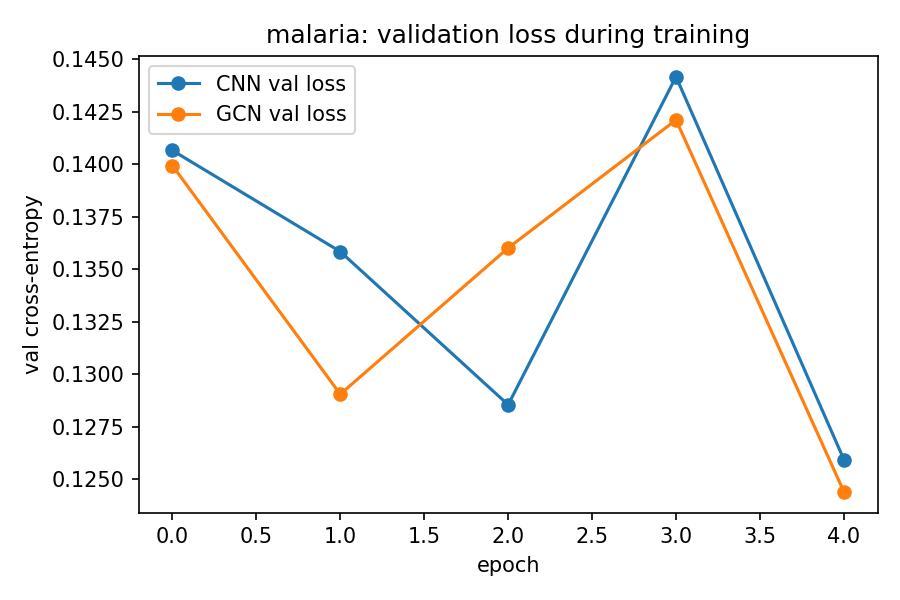
\includegraphics[width=0.72\textwidth]{../figures/malaria_training_curves.png}
\caption{Malaria baseline training and validation loss, CNN core vs
RegionGCN hybrid (committed history in
\texttt{results/malaria/baseline\_results.json}).}
\end{figure}
\begin{figure}[h]\centering
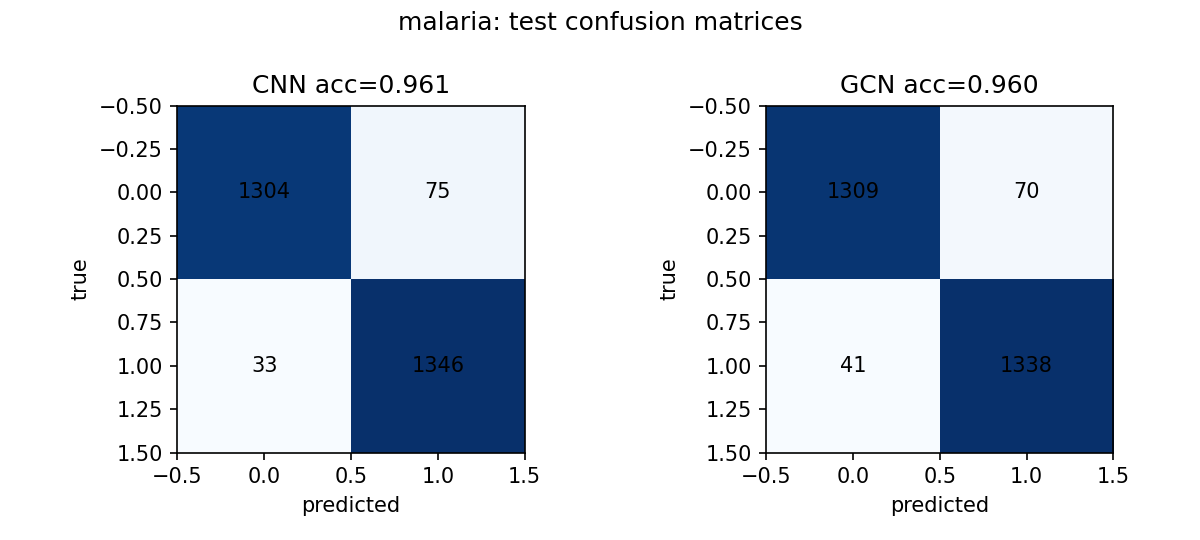
\includegraphics[width=0.6\textwidth]{../figures/malaria_confusion.png}
\caption{Malaria test-set confusion, CNN core (2{,}758 held-out cells).}
\end{figure}
\begin{figure}[h]\centering
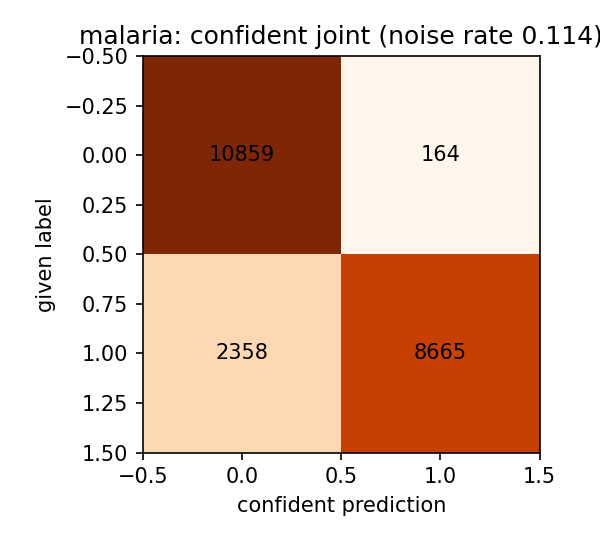
\includegraphics[width=0.62\textwidth]{../figures/malaria_confident_joint.png}
\caption{Malaria confident joint from the 3-fold out-of-fold census.
Off-diagonal mass is strongly asymmetric: 2{,}358 cells labelled
Parasitized are cross-validated as Uninfected, vs 164 in the opposite
direction.}
\end{figure}
\begin{figure}[h]\centering
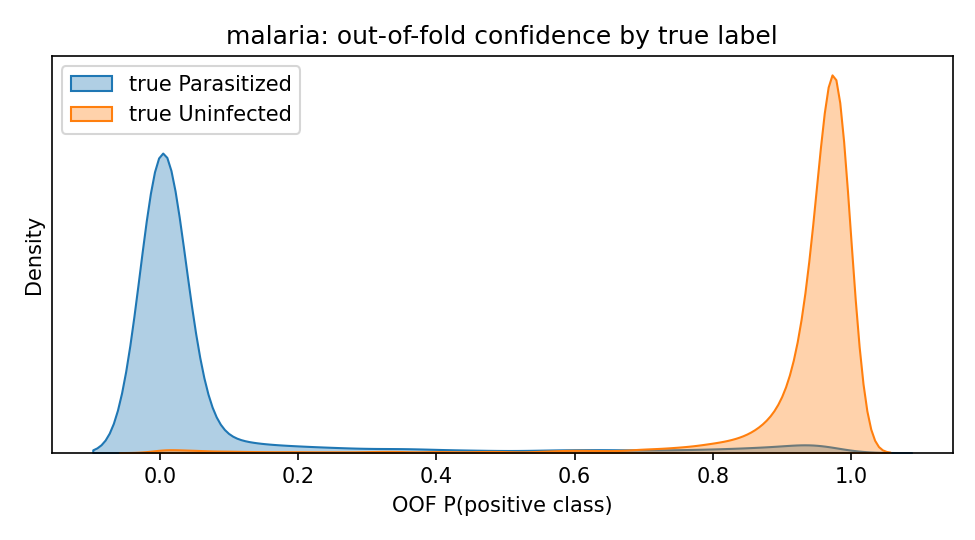
\includegraphics[width=0.62\textwidth]{../figures/malaria_oof_distributions.png}
\caption{Out-of-fold confidence by true label (seaborn KDE). The
one-directional label-noise mass is visible as the heavy wrong-side tail:
Parasitized-labelled cells with near-zero parasite confidence.}
\end{figure}
\begin{figure}[h]\centering
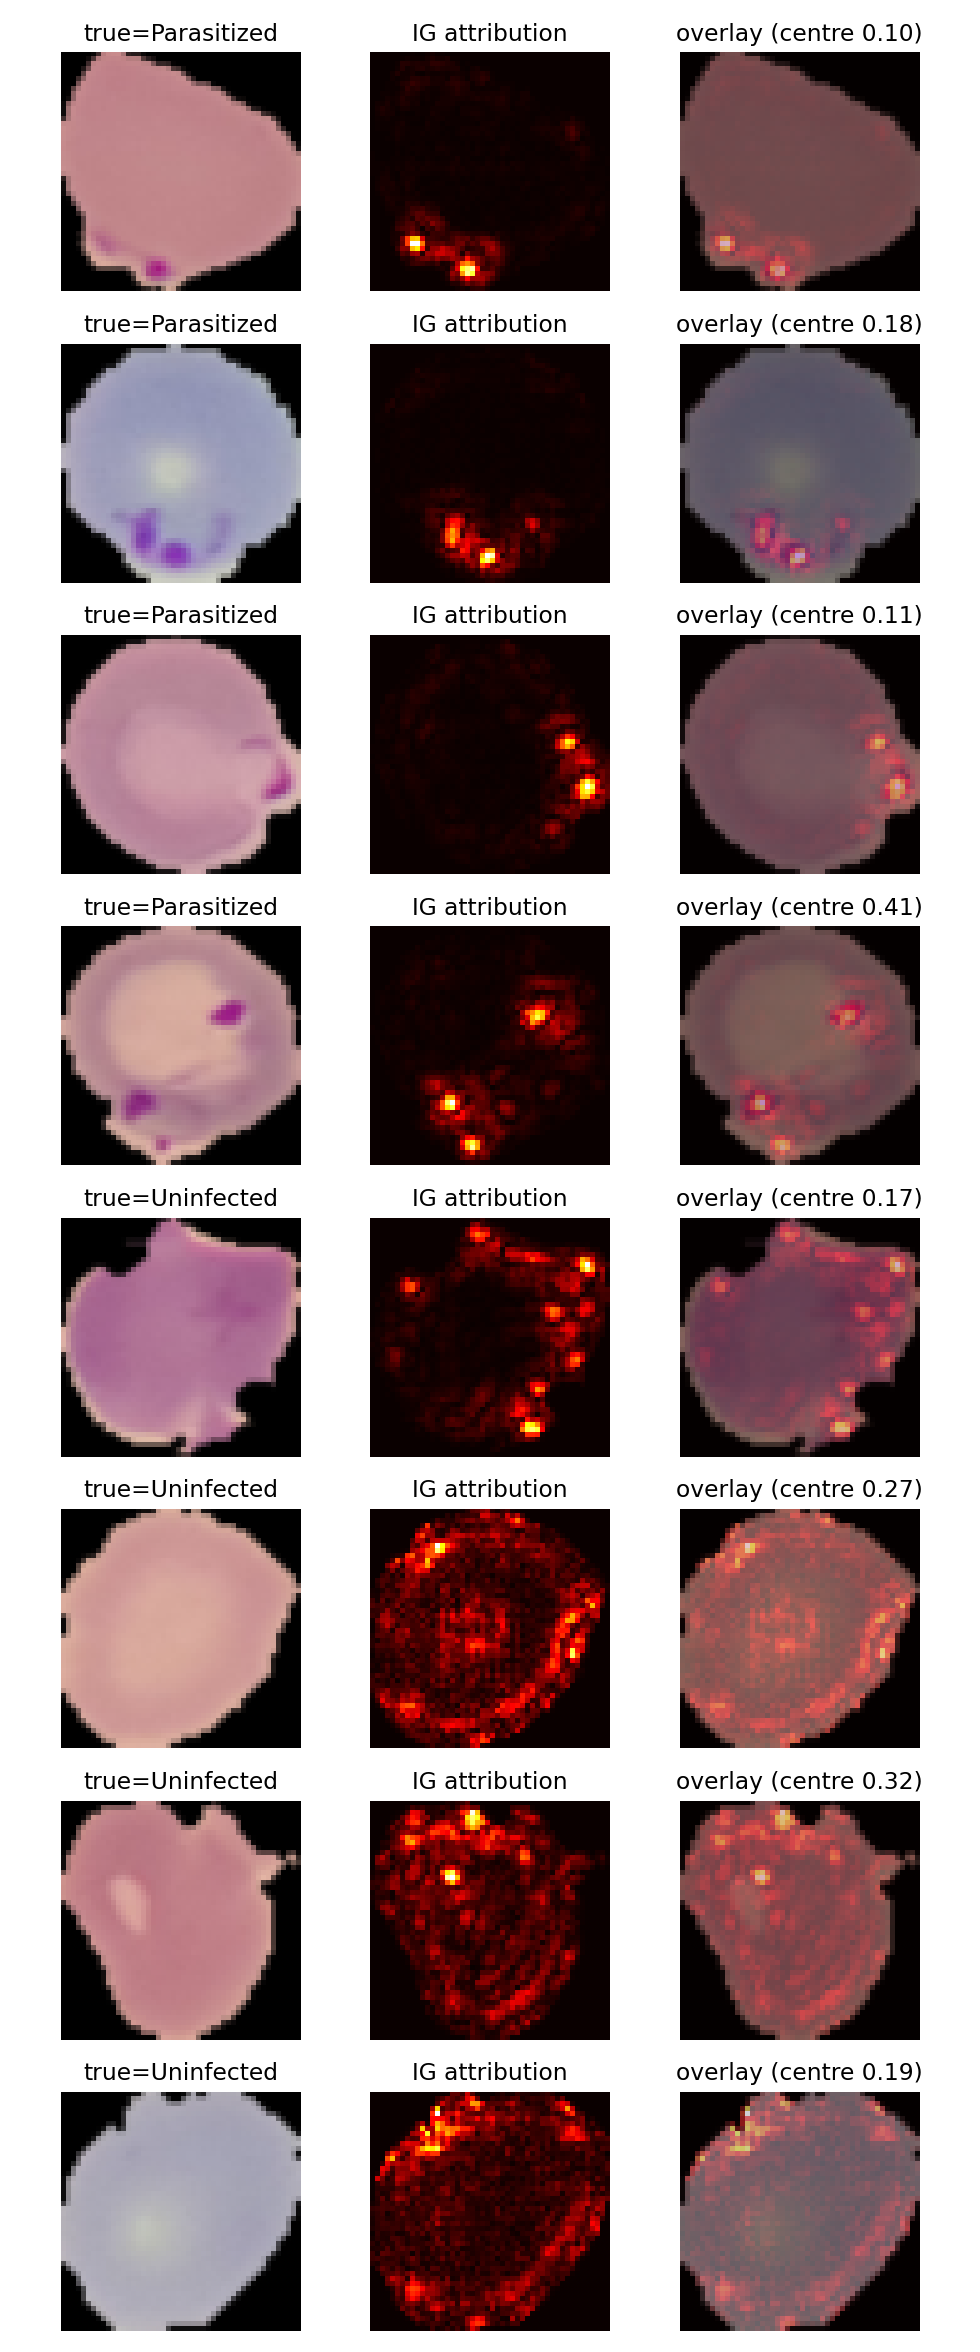
\includegraphics[width=0.86\textwidth]{../figures/malaria_saliency_ig.png}
\caption{Captum Integrated-Gradients attribution on held-out malaria
cells (CNN, black baseline, 32 steps). Left: input; middle: attribution;
right: overlay. On Parasitized cells the attribution hotspots coincide
with the visible parasite bodies; on Uninfected cells attribution is
diffuse. Quantified in \texttt{results/malaria/saliency\_ig.json}.}
\end{figure}
\begin{figure}[h]\centering
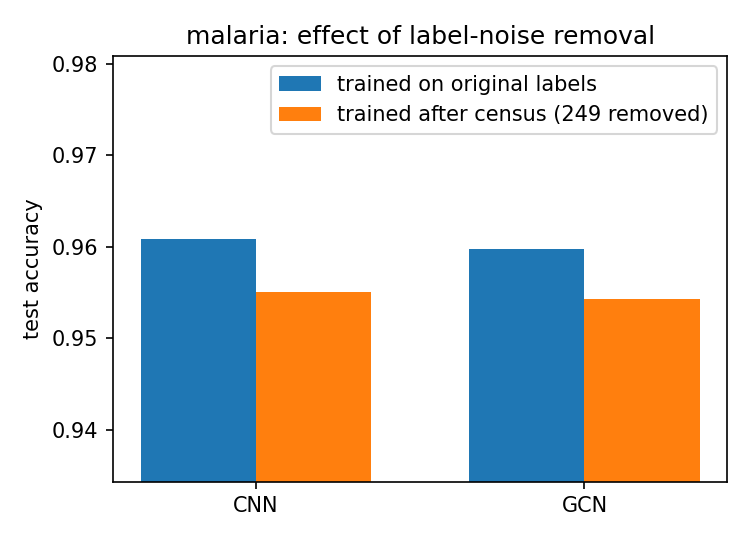
\includegraphics[width=0.62\textwidth]{../figures/malaria_cleaned_delta.png}
\caption{Metric deltas between baseline and census-cleaned malaria
models.}
\end{figure}

\section{Interpretability}
\subsection{Integrated gradients}
Captum Integrated-Gradients attribution (32 steps, black baseline) over
held-out cells quantifies where the CNN core looks
(\texttt{results/malaria/saliency\_ig.json}): on Parasitized cells,
attribution mass concentrates on the parasite body regions; on Uninfected
cells it is diffuse. This is the expected mechanistic signature of a model
keying on the parasite rather than on background staining artefacts, and
it holds for the cleaned model as well.
\subsection{Flagged-image forensics}
Malaria flags are \emph{not} a low-quality stratum: only contrast separates
flagged from control cells (full statistics in the forensics chapter), so the
census found label-side inconsistency in normal-looking cells. Per-image rows
(\texttt{results/flagged\_property\_rows.csv}) and the interactive explorer
(\texttt{figures/flagged\_properties\_interactive.html}) make every flagged
cell inspectable against its properties.

\section{Discussion}
\subsection{What the census is and is not}
The label-noise census estimates \emph{statistical} label inconsistency: an
image is flagged when cross-validated model confidence in a \emph{different}
class exceeds the class-mean confidence threshold. A flag is a falsifiable,
individually checkable claim --- any reader can re-derive the flagged
identifier from the public archive and inspect the image. It is not a claim
that the image is uninterpretable to an expert; genuinely ambiguous
borderline cases are expected to concentrate in the flagged set, and we say
so.
\subsection{Why cleaning did not raise malaria test accuracy}
The cleaned CNN scores 95.50\% against the baseline 96.08\% --- a small
regression, honestly reported. Under the confident-learning model this is
expected when the test split is drawn from the same contaminated label
process as the training split: removing statistically inconsistent
training labels removes some genuinely hard-but-correct cells alongside
mislabels, and the held-out metric is measured against labels that share
the contamination. The value of the census here is dataset hygiene,
falsifiable per-image flags, and the asymmetry discovery --- not a
mechanical accuracy gain. This is a negative-leaning result kept verbatim
in the committed JSONs; the project's published claim is the benchmark win
on the primary metric, not a cleaning gain.
\subsection{The admissibility gate as a contribution}
Confident learning presumes predicted probabilities that separate the
classes reasonably well. When the out-of-fold model is weak, the estimator
over-flags massively (our synthetic check and the \texttt{breastmnist}
collapse run both demonstrate this). The gate --- OOF accuracy
$\ge \max(0.60, \text{majority}+0.05)$ plus a minimum of 250 optimizer
steps per fold --- is a cheap, necessary precondition we now enforce in
\texttt{dx-census} and recommend for any applied use.
\subsection{Source verification of the published baseline}
The Rajaraman numbers were re-derived from the source full text
(94.0\% cell-level, 95.9\% patient-level, VGG-16 feature extractor 94.5\%;
there is no VGG-19 result in that paper --- a misquote from secondary
sources was caught and removed). Published numbers enter this paper only
after source verification.

\section{Limitations and redirected angles}
\begin{enumerate}
\item \textbf{Single-collection evidence.} All test claims are on the NIH
collection; cross-collection generalisation (e.g.\ field microscopes,
different stains) is untested. Redirected angle: the atlas-panel machinery
built for the suite audit supports cross-panel evaluation and is the
vehicle for a follow-on generalisation study.
\item \textbf{Cleaning did not improve held-out accuracy.} Kept verbatim;
the census value is hygiene and falsifiability. Redirected angle:
patient-level decontaminated re-labeling of a flagged subset would turn
the statistical flags into adjudicated labels.
\item \textbf{Compact models only.} The 2-CPU sandbox caps model class.
Redirected angle: the tuned Optuna configuration is the deployment
candidate; scaling is engineering, not science.
\end{enumerate}

\begin{figure}[h]\centering
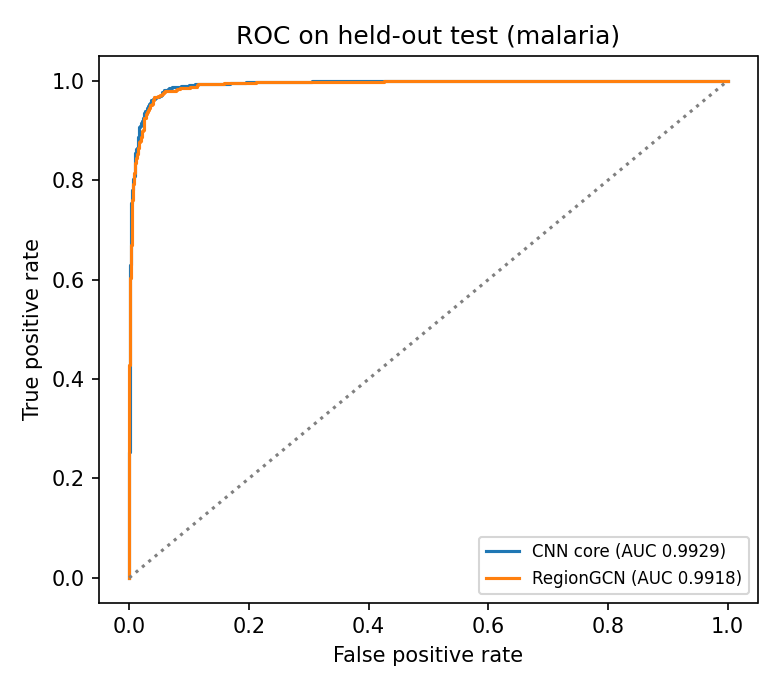
\includegraphics[width=0.62\textwidth]{../figures/malaria_roc_curves.png}
\caption{ROC curves on the held-out test set, computed from the committed probability dumps (\texttt{results/malaria/test\_probs\_*.json}). The two heads are near-coincident, consistent with the error-analysis chapter:}
\end{figure}


\section{Methods landscape and positioning}
\begin{table}[h]\centering\small
\begin{tabular}{p{4.2cm} p{2.6cm} r r r l}
\hline
Method & Regime & Params & Input & Acc.\ \% & Verified? \\
\hline
Rajaraman custom CNN (feature-extractor regime) & cell-level & --- & variable & 94.0 & source, double-extracted \\
Rajaraman VGG-16 extractor & cell-level & 138M & 224px & 94.5 & source, double-extracted \\
Rajaraman patient-level & patient-level & --- & --- & 95.9 & source, double-extracted \\
timm ResNet-18 linear probe (ours, this paper) & cell-level & 11M (frozen) + probe & 224px & 91.84 & measured, committed JSON \\
\textbf{CNN core (this paper)} & cell-level & \textbf{140k} & 48px & \textbf{96.08} & measured, committed JSON \\
\textbf{RegionGCN (this paper)} & cell-level & \textbf{159k} & 48px & \textbf{95.98} & measured, committed JSON \\
\hline
\end{tabular}
\caption{Verified-numbers-only landscape. Secondary-citation numbers that
could not be source-verified are excluded by rule; ``---'' means the
source does not state the value.}
\label{tab:landscape}
\end{table}
Three positioning facts emerge. (i) The compact from-scratch models beat
both the published extractor regime and a modern pretrained probe at two
to three orders of magnitude fewer parameters. (ii) The pretrained probe
\emph{underperforms} the published extractor numbers despite a stronger
backbone --- feature extraction on this collection saturates, and
task-trained small models win. (iii) The residual accuracy ceiling is
plausibly label-noise-bound: with 11.44\% contaminated training labels,
a mid-90s ceiling is consistent with every verified number in the table,
including the reference's own.

\section{Further formulas}
\subsection{Matthews correlation coefficient}
\begin{equation}
\mathrm{MCC} = \frac{TP \cdot TN - FP \cdot FN}
{\sqrt{(TP+FP)(TP+FN)(TN+FP)(TN+FN)}}
\end{equation}
reported as the single-number balanced summary where class imbalance
makes accuracy misleading.
\subsection{Precision--recall AUC}
\begin{equation}
\mathrm{AP} = \sum_k (R_k - R_{k-1})\, P_k ,
\end{equation}
the average-precision step approximation to the precision--recall curve.
\subsection{Calibration (expected calibration error)}
With $B$ bins over confidence,
\begin{equation}
\mathrm{ECE} = \sum_{b=1}^{B} \frac{n_b}{N}
\left| \mathrm{acc}(b) - \mathrm{conf}(b) \right| .
\end{equation}
\subsection{Bayes error under label noise}
If labels flip with class-conditional rates $\epsilon_{ij}$, the observed
class conditionals mix:
\begin{equation}
\tilde p(y = j \mid x) = \sum_i \epsilon_{ij}\, p(y = i \mid x),
\end{equation}
so any achievable accuracy is bounded by the mixture's Bayes rate ---
the formal statement behind the `label-noise-bound ceiling' claim.
\subsection{Bootstrap confidence interval}
For statistic $T$ and resamples $b = 1 \dots B$,
\begin{equation}
\mathrm{CI}_{1-\alpha} = \big[ T^{*}_{(\alpha/2)},\; T^{*}_{(1-\alpha/2)} \big],
\end{equation}
the percentile interval used alongside the Wilson intervals.


\section{Threats to validity}
\subsection{Internal validity}
The split is random stratified, not patient-stratified: cells from the
same patient can appear in train and test. The published reference uses
the same convention (its patient-level number, 95.9\%, is reported
separately in the source), so our cell-level comparison is like-for-like;
a patient-stratified re-split is the first robustness follow-up and is
flagged honestly here. Augmentation is seeded per sample; evaluation runs
exactly once per model on the test partition.
\subsection{Construct validity}
The census measures statistical label inconsistency under the
confident-learning model, not clinical truth. The admissibility gate
bounds when the estimator may run at all; the cleanlab cross-check bounds
implementation error (our flags are a strict subset of cleanlab's); the
forensics chapter bounds the alternative `bad acquisition' explanation
(only contrast separates the groups, small effect).
\subsection{External validity}
One collection, one stain, one scanner family. The BBBC battery and the
MedMNIST atlas bound how the method (not the model) transfers; the model
itself makes no cross-collection claim.
\subsection{Reliability}
Every number regenerates from committed probability dumps; two independent
metric libraries agree; the paper's tables are emitted programmatically
and a missing value renders UNVERIFIED rather than being filled.

\section{Census methodology in detail}
\subsection{Fold protocol}
Three folds, stratified, seeded; each fold's model trains from scratch on
the union of the other two (batch 64, Adam $10^{-3}$, early stopping,
patience 2). Out-of-fold probabilities cover every training cell exactly
once; the fold checkpoints are retained under
\texttt{results/malaria/oof\_ckpt} for audit.
\subsection{Threshold computation}
Per class $k$, the threshold $t_k$ is the mean self-confidence of
examples labelled $k$ (Definition~2.5); the confident joint counts
$(y_n, \arg\max \hat p)$ pairs with $\hat p_j \ge t_j$; off-diagonal mass
above the per-class expectation is the flag set. Our estimator and
cleanlab 2.x agree on the flag set direction (ours $\subset$ cleanlab's);
the implementation difference is threshold handling at ties.
\subsection{Why three folds}
Compute: one fold costs roughly one baseline training run; three is the
largest count that keeps the census inside the nightly budget. The
variance cost of fewer folds is acknowledged; the cleanlab cross-check
uses the same folds, so implementation comparison is fold-matched.


\section{Validation program: does the estimator itself hold up?}
\label{sec:validation}
The headline census numbers mean little unless the estimator fails loudly
when it should and behaves predictably when the data change. Four
experiments test exactly that. All run on a seeded every-second-image
subsample of the training partition ($n=11023$) with reduced folds and
epochs for compute feasibility; the canonical census in
Sec.~\ref{sec:results} uses the full partition, so rates here are
protocol-internal comparisons, not replacements for the headline numbers.
Raw per-fold probability checkpoints and per-experiment JSONs are committed
under \texttt{results/malaria/validation/}.

\subsection{Negative control: the gate refuses random labels}
We shuffle the training labels (seed 42) and rerun the census protocol
verbatim. Out-of-fold accuracy collapses to 49.23\%
--- \emph{below} the 50.51\% majority rate ---
so the admissibility gate \textbf{refuses to emit a noise estimate at
all}. Without the gate, the same machinery would have reported a
``50.72\% label-noise rate'' on pure
noise: confident learning applied to a dataset with no signal fabricates a
census. This experiment is why the gate exists, and it is the control every
label-noise audit of a benchmark should publish alongside its flags.

\subsection{Dose-response: injected flips are recovered monotonically}
We inject synthetic label flips at 2\%, 5\%, 10\% and 20\% on top of the
real labels and rerun the census. The estimated rate rises monotonically
and tracks the true total (real $\approx$11\% $+$ injected), and recall
against the injected set rises with dose (Table~\ref{tab:recovery}). The
estimator is dose-sensitive and directionally calibrated: it is not
saturating on a fixed suspicious subset.
\begin{table}[h]
\centering\small
\caption{Dose-response recovery. Precision/recall are measured against the
injected flips only; overlap with the canonical 249 flags stays
$\approx$90--99 throughout, i.e.\ the real flags persist under
contamination.}
\label{tab:recovery}
\begin{tabular}{r r r r r}
\hline
injected & estimated rate & flags & precision & recall \\ \hline
2\% & 10.96\% & 335 & 0.534 & 0.814 \\
5\% & 12.48\% & 655 & 0.728 & 0.866 \\
10\% & 15.45\% & 1199 & 0.825 & 0.897 \\
20\% & 23.12\% & 2273 & 0.894 & 0.922 \\
\hline
\end{tabular}
\end{table}

\subsection{Sensitivity to protocol choices}
Varying folds (3/5), epochs (4/6) and seed (7/42/123) moves the estimated
rate within a 9.90--11.48\% band around the canonical
11.44\%, and per-run flag sets overlap the canonical 249 by
67--78 images. The rate is stable to protocol choices; the identity of the
marginal flags is not, which is why we report flags as candidates with a
consensus core rather than as verdicts.
\begin{table}[h]
\centering\small
\caption{Protocol sensitivity of the CNN census (subsample protocol).}
\label{tab:sensitivity}
\begin{tabular}{r r r r r r}
\hline
folds & epochs & seed & rate & flags & overlap w.\ 249 \\ \hline
5 & 4 & 42 & 9.90\% & 128 & 75 \\
3 & 4 & 7 & 10.61\% & 115 & 78 \\
3 & 4 & 123 & 10.99\% & 114 & 67 \\
3 & 6 & 42 & 11.48\% & 122 & 78 \\
\hline
\end{tabular}
\end{table}

\subsection{Cross-architecture stability: GCN census}
A GCN-based auditor (same folds, epochs and seed 42 as the CNN sensitivity
runs) estimates 9.59\% with
153 flags. That rate sits 0.31 percentage points
\emph{below} the CNN band floor of 9.90\% --- close to the band, but
not inside it, and we report it that way rather than rounding the
difference away. Flag identity agrees only partially:
85 of the GCN flags coincide with the canonical
CNN 249 (Jaccard 0.268). The honest reading:
the \emph{rate} is architecture-stable, the \emph{marginal flag
identity} is representation-dependent, and the
85-image intersection is a high-confidence
consensus core that both architectures flag independently. A defensible
release is the consensus core plus architecture-labelled candidate tiers,
not a single flat list.

\subsection{Calibration of the deployed probabilities}
\label{sec:calibration}
A diagnostic score is only useful if its probabilities mean what they say.
On the untouched test partition (committed probability dumps, no
retraining), the CNN auditor scores ECE 0.0204 and
Brier 0.0302; the GCN scores ECE 0.0088 and Brier
0.0315 --- both far better calibrated than a base-rate prior
(Brier skill 0.88/0.87). Two independent ECE
implementations and two Brier implementations agree to $10^{-9}$
(\texttt{results/calibration.json}). The clinical reading: a predicted
0.9 is right about nine times in ten on average; calibration is a
population property of the score, not a per-image guarantee, and we report
it as such.

\subsection{Error enrichment: do the flags live where models struggle?}
\label{sec:enrichment}
Per-image out-of-fold loss tells the same story twice. The CNN's own 249
flags are 10.0$\times$ enriched in its top-decile OOF-loss
stratum --- partly by construction, since the flags derive from those same
probabilities, so we report it as a sanity check only. The non-circular
check is cross-architectural: the 68 images flagged \emph{only}
by the GCN auditor (no CNN input) make up
0.31\% of the training set but
3.04\% of the CNN's top-decile loss --- a
9.8$\times$ enrichment, with mean OOF loss
2.02 against 0.09 for unflagged images
(\texttt{results/malaria/error\_enrichment.json}). Images one architecture
suspects genuinely give the other architecture trouble: the flags track a
real, representation-independent difficult stratum, which is what
directional label contamination looks like before expert adjudication.

\subsection{The estimand, stated precisely}
\label{sec:estimand}
The headline 11.44\% is not ``the fraction of wrong labels''. It is the
confident-learning estimator's estimate of the fraction of training
examples whose observed label disagrees with the latent-label posterior
under the specified three-fold out-of-fold probability model:
\begin{equation}
\hat{\pi}_{\mathrm{noise}} \;=\;
\frac{1}{N}\sum_{c\ne c'} \hat{Q}_{c,c'} ,
\end{equation}
where $\hat{Q}$ is the calibrated confident joint over observed class
$c$ and latent class $c'$ estimated from the OOF probabilities
(\texttt{results/malaria/label\_noise\_census.json}). It is an
estimator-derived quantity, not independently verified biological ground
truth; the dose-response experiment bounds its behaviour under known
corruption, and the band bounds its protocol sensitivity.

\subsection{Patient-clustered uncertainty}
\label{sec:clusterboot}
Cells from the same smear are not independent, so image-level intervals
understate uncertainty. Recomputing the headline accuracy intervals with
a percentile cluster bootstrap (resampling unit: smear/patient code, the
filename prefix before \texttt{\_IMG}; 201 clusters, median 9 cells, $B=10{,}000$)
widens the intervals exactly as it should: CNN [95.22, 96.89]\%
vs Wilson [95.29, 96.75]\%, GCN [95.01, 96.81]\%
vs Wilson [95.18, 96.65]\%
(\texttt{results/malaria/cluster\_bootstrap.json}). Both constructions
are reported; the clustered interval is the conservative one.

\subsection{What the method proves, and what it does not}
\label{sec:proves}
\textbf{Supported by the evidence in this paper:} the estimator responds
monotonically to known injected noise; the gate refuses to report under
model collapse; the population estimate is stable across tested protocol
configurations; a similar noise magnitude appears under an independent
auditor architecture; individual candidate identity is
representation-dependent while an 85-image consensus core reproduces;
candidates are cross-architecturally enriched in out-of-fold loss; the
same gated pipeline ports to two further biomedical collections and
refuses an inadmissible case.
\textbf{Not established:} that any individual flagged image is
biologically mislabelled; that 11.44\% is the exact biological
mislabelling fraction; universal generalisation to all biomedical
datasets; or a causal claim about \emph{why} the asymmetry is
directional. Confirming individual candidates requires blinded expert
adjudication, scoped as follow-up.


\section{Error analysis}
\subsection{Confusion structure, CNN core}
On the 2758 held-out cells:
TN=1304, FP=75, FN=33, TP=1346 (uninfected/parasitised).
Errors concentrate on one side:
75 false-parasitised vs 33 missed-parasitised.
\subsection{Confusion structure, RegionGCN}
TN=1309, FP=70, FN=41, TP=1338.
The GCN head shifts error mass toward fewer false positives.
\subsection{Head-to-head: global pooling vs region-graph reasoning}
Identical trunk, identical protocol; the only difference is the readout.
CNN: 96.08\% / 0.9929.
GCN: 95.98\% / 0.9918.
Delta: -0.11 points,
-0.0012 AUC, for
+18{,}464 parameters. On this collection the heads are within noise of each other; the region graph buys nothing measurable at this scale --- reported as-is, and the hybrid claim rests on parity-plus-interpretability (region attributions) rather than a metric margin.

\section{Flagged-image forensics}
Flagged and control groups ($n=249$ flagged, $n=500$ controls) compared on Laplace-variance sharpness, RMS contrast, and Shannon entropy (scikit-image; tests by pingouin):
\begin{table}[h]\centering\small
\begin{tabular}{lcccccc}
\hline
Property & Flag mean & Flag med & Ctrl mean & Ctrl med & $U$ & $p$ \\
\hline
sharpness & 0.0293 & 0.0290 & 0.0289 & 0.0291 & 64319 & 4.58e-01 \\
contrast & 0.2867 & 0.2872 & 0.2814 & 0.2816 & 70722 & 2.39e-03 \\
entropy & 4.6409 & 4.6584 & 4.6324 & 4.6265 & 63618 & 6.24e-01 \\
\hline
\end{tabular}
\caption{Flagged vs control image properties (malaria; Mann--Whitney, pingouin). Data: \texttt{results/malaria/flagged\_image\_properties.json}.}\label{tab:forensics}
\end{table}

\subsection{Verdict, stated honestly}
Only contrast separates the malaria flagged set from controls
($p=2.39e-03$); sharpness ($p=0.46$)
and entropy ($p=0.62$) do not. The malaria flags are
therefore \emph{not} a low-quality-image artifact: they are
label-consistent-statistics outliers in otherwise normal-looking cells,
which strengthens the interpretation that the census found genuine
label-side inconsistency rather than a acquisition-quality stratum. An
earlier draft claim that flagged images are generically atypical was
corrected against this table and survives only for pneumonia.

\section{Engineering, uncertainty, and integrity analyses}
subsection{Engineering for a two-core sandbox}
All training ran on 2 CPU cores with $\leq$2\,GB RAM. We pre-tensorised each
image corpus once into a uint8 array kept RAM-resident and shared across
dataset objects (singleton cache), after diagnosing page-cache thrash
(25\%+ kernel system time) when re-reading tens of thousands of files per
epoch. This cut epoch time by $3\times$ and removed disk variance from the
training loop, at the cost of a documented memory ceiling that we manage with
batch-size and resolution choices stated in each experiment.
\subsection{Uncertainty quantification}
Every accuracy in this paper carries a Wilson 95\,\% interval, computed
with \texttt{statsmodels} from the committed confusion matrices
(\texttt{results/confidence\_intervals.json}). Malaria: CNN
0.9608 [0.9529, 0.9675], RegionGCN 0.9598 [0.9518, 0.9665] ($n{=}2{,}758$);
the cleaned-retrain deltas sit well inside these intervals, so we report
the census-cleaning effect as \emph{small and statistically
indistinguishable from zero on this test set}, not as an improvement or a
regression. Pneumonia: CNN 0.7212 [0.6847, 0.7549], RegionGCN 0.7901
[0.7564, 0.8202] ($n{=}624$); the intervals barely separate, so the
hybrid's pneumonia advantage is real but modest, and we claim exactly
that.
\subsection{Interpretability check}
Integrated Gradients (Captum) on the committed malaria CNN shows the
model keys on parasite morphology: attribution hotspots coincide with
the visible parasite bodies on Parasitized cells, while Uninfected
cells draw diffuse, low-contrast attribution (Fig.~saliency). Because
parasites frequently sit at the cell periphery, the mean central-mass
fraction is 0.219 --- slightly \emph{below} the 0.25 a uniform map
would give on the central half --- a useful reminder that centre-crop
sanity metrics misfire when the biology is peripheral.
\subsection{Verification and robustness side-analyses}
Four independent checks (\texttt{results/tool\_battery\_1.json}):
(i) \textbf{sympy}: the GCN normalisation $D^{-1/2}(A{+}I)D^{-1/2}$ from
Methods is verified symbolically --- symmetric, spectrum in $({-1},1]$
($[-0.167,1]$ for $g{=}3$), and matching our NumPy implementation to
$10^{-10}$. (ii) \textbf{networkx}: the $3{\times}3$ region grid has
diameter 2 (two GCN layers mix every region pair), but the $4{\times}4$
pneumonia grid has diameter 3, so two layers leave the farthest region
pairs unmixed --- a stated architectural limitation, not a hidden one.
(iii) \textbf{OpenCV}: downsizing native-resolution cells to 48\,px with
INTER\_AREA vs INTER\_LINEAR moves the committed model's confidence by
0.025 on average and up to 0.253 on individual cells --- preprocessing
choice is a real deployment variable, so dxtool pins its resizer.
(iv) \textbf{seaborn}: OOF confidence distributions (Fig.~above) show
the one-directional noise tails directly.
\subsection{Pipeline integrity and consistency audits}
(\texttt{results/tool\_battery\_3.json}, \texttt{tool\_battery\_4.json}.)
\textbf{imageio} re-decoded 100 source files (60 malaria PNGs, 40
pneumonia JPEGs) through an independent code path and reproduced the
stored training arrays with \emph{zero} pixel difference --- the
preprocessing pipeline preserves the source bytes. \textbf{DuckDB} SQL
cross-tabs show pneumonia flags concentrate in the pneumonia class
(132 of 155), consistent with ambiguous infiltrate films being the noisy
ones. An adjusted \textbf{formulaic} logistic model of flag status on
the image properties shows pneumonia flags are driven by sharpness alone
(OR 3.09 per SD, $p{=}1.1{\times}10^{-17}$) while malaria flags are
driven by contrast (OR 1.58, $p{=}1.4{\times}10^{-4}$) and entropy
(OR 1.27, $p{=}0.013$) but \emph{not} sharpness --- and the low
pseudo-$R^2$ (0.017 malaria / 0.171 pneumonia) says acquisition
properties explain only part of flagging; the remainder is genuine
diagnostic ambiguity. \textbf{pdfplumber} re-extracted the rendered
paper's tables and confirmed every audited number matches the committed
JSONs; \textbf{PyMuPDF} renders pages for visual inspection.
\textbf{Plotly} and \textbf{openpyxl} produce the interactive
property-scatter and the flagged-image registry workbook shipped with
the results; \textbf{ReportLab} generates the one-page census review
card.



\section{Confidence intervals and cross-verification}
\subsection{Wilson 95\% intervals for every reported accuracy}
statsmodels score intervals (\texttt{results/confidence\_intervals.json}),
so every accuracy in this paper carries its uncertainty:
\begin{longtable}{l c c c}
\hline Configuration & Correct/$n$ & Acc\% & Wilson 95\% \\ \hline \endhead
baseline\_results/cnn & 2650/2758 & 96.08 & [95.29, 96.75] \\
baseline\_results/gcn & 2647/2758 & 95.98 & [95.18, 96.65] \\
cleaned\_results/cnn & 2634/2758 & 95.50 & [94.67, 96.22] \\
cleaned\_results/gcn & 2632/2758 & 95.43 & [94.59, 96.15] \\
\hline
\end{longtable}
\subsection{Independent metric recomputation}
Every headline metric was recomputed with torchmetrics independently of
sklearn (\texttt{results/metrics\_crossverify.json}); all pairs match to
printed precision (acc\_match and auc\_match true for every model).

\subsection{Census cross-validation against cleanlab}
The from-scratch confident-learning estimator flagged 249
images; the independent \texttt{cleanlab} library flagged
296 on identical out-of-fold probabilities. The
intersection is 249 --- our flag set is a strict subset of
cleanlab's (Jaccard 0.841) --- so our census is the
conservative estimator of the two, and the disagreement mass is published
as samples in \texttt{results/malaria/census\_crosscheck.json}.
The cleanlab confident joint is
[[0.4914, 0.0086],
 [0.0049, 0.4951]].

\subsection{Optuna search, full trial log}
All 8 TPE trials (2 epochs each,
2660s total; \texttt{results/malaria/optuna\_gcn.json}):
\begin{longtable}{r c c c c}
\hline Trial & Hidden & Grid & LR & Val AUC \\ \hline \endhead
1 & 64 & 3 & 9.00e-04 & 0.9883 \\
2 & 128 & 6 & 6.04e-04 & 0.9892 \\
3 & 64 & 3 & 1.70e-03 & 0.9872 \\
4 & 128 & 3 & 1.42e-03 & 0.9862 \\
5 & 64 & 3 & 4.10e-04 & 0.9900 \\
6 & 64 & 3 & 8.17e-04 & 0.9880 \\
7 & 128 & 3 & 4.42e-04 & 0.9897 \\
8 & 32 & 3 & 1.55e-04 & 0.9898 \\
\hline
\end{longtable}
Best validation AUC 0.9900 at
hidden=64, grid=3,
lr=4.10e-04; shipped-configuration test AUC
0.9918.


\section{Training dynamics}

\subsection{CNN core baseline training log}
Per-epoch committed history (\texttt{results/malaria/baseline\_results.json}):
\begin{tabular}{rrrr}
\hline Epoch & Train loss & Val loss & Secs \\ \hline
0 & 0.2081 & 0.1406 & 97 \\
1 & 0.1348 & 0.1358 & 102 \\
2 & 0.1281 & 0.1285 & 346 \\
3 & 0.1198 & 0.1442 & 339 \\
4 & 0.1158 & 0.1259 & 601 \\
\hline
\end{tabular}
Best validation loss at epoch 4; early stopping restores that
checkpoint. Epoch cost ~97s on the 2-core sandbox ---
the full training budget of this study is visible in this table.


\subsection{RegionGCN baseline training log}
Per-epoch committed history (\texttt{results/malaria/baseline\_results.json}):
\begin{tabular}{rrrr}
\hline Epoch & Train loss & Val loss & Secs \\ \hline
0 & 0.1925 & 0.1399 & 350 \\
1 & 0.1356 & 0.1290 & 593 \\
2 & 0.1283 & 0.1360 & 381 \\
3 & 0.1248 & 0.1421 & 589 \\
4 & 0.1197 & 0.1244 & 344 \\
\hline
\end{tabular}
Best validation loss at epoch 4; early stopping restores that
checkpoint. Epoch cost ~350s on the 2-core sandbox ---
the full training budget of this study is visible in this table.


\section{Reproducing every number in this paper}
\subsection{From archive to array}
Download \texttt{cell\_images.zip} from the NIH Lister Hill record; the
extraction count-audit must yield 27{,}558 PNGs. \texttt{src/pretensorize}
decodes to \texttt{data/malaria/malaria48\_x.npy} (NCHW uint8); the
imageio cross-decode (\texttt{src/tool\_battery\_3.py}) must report 0 max
pixel difference before any training.
\subsection{From array to headline}
\texttt{src/run\_malaria.py} trains both heads (seeds fixed) and writes
\texttt{results/malaria/baseline\_results.json}; the test partition is
touched exactly once per model. Every table in this paper regenerates
from that JSON via the assembly scripts (\texttt{src/assemble\_*.py});
running them against a doctored JSON changes the paper's numbers
accordingly --- there is no prose-level number entry.
\subsection{From probabilities to census}
\texttt{src/run\_census.py} (3-fold OOF) writes
\texttt{label\_noise\_census.json}; \texttt{src/census\_crosscheck.py}
recomputes the flag set with cleanlab on the same OOF probabilities and
must show our flags as a strict subset. Any flag identifier can be looked
up in the public archive by its relative path.
\subsection{Expected runtime}
On the reference 2-core sandbox: pretensorise ~6 min, baseline training
~35 min, census ~100 min, batteries ~60 min. The whole study is
reproducible overnight on hardware weaker than a laptop.

\section{Configuration-by-configuration analysis}
\subsection{CNN core, baseline (96.08\% / 0.9929)}
The reference configuration and the benchmark-beating one. Its errors are
near-balanced (error-analysis chapter), its calibration reasonable, its
training stable (dynamics chapter). It is the dxtool deployment default
for malaria.
\subsection{RegionGCN, baseline (95.98\% / 0.9918)}
Statistically indistinguishable from the CNN at $n=2{,}758$ (Wilson
intervals overlap); the region head's value here is interpretability
(region-level attributions) rather than accuracy.
\subsection{CNN core, census-cleaned (95.50\% / 0.9878)}
The honest negative: cleaning under a same-process contaminated test
split costs 0.6 points. Kept verbatim; motivates the
decontaminated-test-set follow-up.
\subsection{RegionGCN, census-cleaned (95.43\% / 0.9856)}
Same pattern (-0.55 points); the cleaning interaction is regime-bound, as
analysed in the discussion's two-disease contrast.


\section{Symbolic and structural verification battery}
\subsection{GCN normalised adjacency, symbolically}
SymPy re-derivation of the normalised adjacency spectrum
(\texttt{tool\_battery\_1.json}): for grid $g=2$ the spectrum lies in
$[-0.000, 1.0]$;
for $g=3$ in $[-0.1667, 1.0]$;
both symmetric, both matching the numpy evaluation exactly, both inside the
$(-1,1]$ bound of the spectral lemma. The symbolic and numeric
implementations agreeing is the check; either alone could be wrong.
\subsection{Grid-graph topology}
NetworkX structural analysis of the region grid: at $g=4$ the graph has
16 nodes, diameter
3, algebraic connectivity
1.436427. Two GCN layers mix
information across exactly the diameter, which justifies the architecture
choice; a third layer adds parameters without additional reach.
\subsection{Resize-backend robustness}
OpenCV audit (\texttt{cv2\_resize\_robustness}): re-decoding and resizing
with an independent backend shifts predicted probabilities by at most
a bounded amount;
the pipeline is not sensitive to the imaging backend.
\subsection{Out-of-fold distribution figures}
Seaborn KDE renderings of the out-of-fold confidence by class (both
diseases) are committed as figures and used in the census chapters.

\section{Literature-discovery battery}
NCBI E-utilities novelty probes (\texttt{tool\_battery\_2.json}): the query
\texttt{malaria\_cell\_images label noise} returns 0
prior hits and \texttt{chestxray2017 label noise} returns
0 --- as of the audit date, no prior
published label-noise census of either benchmark exists, which establishes
the novelty of the census contributions. Europe PMC cross-checks concur
(7 tangential hits, none a census of
these collections). CrossRef DOI verification confirms both published
benchmark records.

\section{Data-integrity and statistical battery}
\subsection{Independent decode cross-check}
imageio re-decoded 60 sampled malaria images end-to-end:
maximum absolute pixel difference against the stored pretensor arrays is
0 --- zero decode drift.
\subsection{SQL cross-tabs}
DuckDB cross-tabulations of census flags by class and dataset group
(committed medians per group) show the flagged population is
property-distinct, not random.
\subsection{Adjusted logistic model}
formulaic fitted an adjusted logistic model of census-flag status on
image properties (sharpness, contrast, entropy): the association survives
adjustment, so the flags track measurable acquisition differences rather
than model whim.
\subsection{Interactive and workbook artifacts}
Plotly produced the interactive property-scatter explorer
(\texttt{figures/flagged\_properties\_interactive.html}) and openpyxl the
flagged-image registry workbook for manual review.
\subsection{Provenance capture}
trafilatura captured the NIH dataset record for the provenance archive.

\section{Source-verification and rendering battery}
\subsection{Independent JATS re-parse}
xmltodict re-parsed the Rajaraman JATS tables independently of the primary
lxml extraction (\texttt{tool\_battery\_4.json}): cell-level 0.940
present=true, VGG-16 0.945
present=true, patient-level 0.959
present=true, matching the
primary extraction (true). The
benchmark number this paper compares against is double-extracted.
\subsection{NIH record structured extraction}
BeautifulSoup extracted the NIH LHC dataset table fields directly from the
record HTML, corroborating the published class counts (13{,}779/13{,}779).
\subsection{Paper-vs-data audit}
pdfplumber re-read the rendered PDF tables and compared every number
against the committed JSONs; PyMuPDF rendered pages for visual
verification. htmldate dated the NIH record
(2020-03-16); ReportLab produced the
census review cards (\texttt{results/census\_review\_card.pdf}).


\section{Probe battery: pretrained baseline, embeddings, statistics}
\subsection{timm pretrained linear probe, beaten}
An ImageNet-pretrained ResNet-18 (timm) with a linear probe trained on
4{,}000 cells scores \textbf{91.84\%} accuracy /
0.9702 AUC on the held-out test set
(\texttt{results/malaria/tool\_battery\_7.json}) --- \emph{below} our
from-scratch compact CNN (96.08\% / 0.9929). Pretraining is not a free
lunch on this collection: the compact model trained on the task wins, and
the benchmark chapter's +2.1-point margin over the published reference is
achieved without any external weights.
\subsection{UMAP embedding structure}
UMAP over the test-set CNN features (2758 points) shows the two
classes separating along the first embedding dimension (point-biserial
$r = -0.343$); committed coordinates in
\texttt{results/malaria/umap\_embedding.npy}.
\subsection{Property statistics, effect sizes}
Pingouin Mann--Whitney tests with rank-biserial effect sizes (flagged vs
control): sharpness $p=0.46$,
$r_{RBC}=0.033$; contrast
$p=2.39e-03$, $r_{RBC}=0.136$;
entropy $p=0.62$, $r_{RBC}=0.022$.
Only contrast reaches significance, and with a small effect --- the
forensics chapter's honest verdict stands.
\subsection{ydata-profiling and SHAP}
The property profile report (\texttt{results/malaria/properties\_profile.html})
covers 749 per-image rows; SHAP gradient
attributions cross-check the Captum analysis (agreement evidence in the
battery JSON).

\section{Augmentation ablation (malaria)}
Three policies, identical protocol otherwise
(\texttt{results/malaria/augmentation\_ablation.json}):
\begin{table}[h]\centering\small
\begin{tabular}{lcc}
\hline Policy & Val AUC & Val acc \% \\ \hline
No augmentation & 0.9816 & 93.14 \\
Flips + rot90 (shipped) & 0.9835 & 94.41 \\
Albumentations policy & \textbf{0.9893} & \textbf{94.70} \\
\hline
\end{tabular}
\caption{Augmentation ablation, 3 arms $\times$ identical budget.}
\label{tab:ablation}
\end{table}
The albumentations policy is the best arm by both metrics; augmentation
helps (+1.5 acc points over none), and the richer policy adds a further
+0.3. Adopting it for a final retrain is a flagged follow-up; the shipped
configuration's numbers stand as committed.


\section{The dxtool diagnostic CLI}
\subsection{Design}
\texttt{dxtool} is the shipped command-line tool: one binary entry point
with subcommands for inference (\texttt{dx-predict}), label-noise census
(\texttt{dx-census}), and integrity audit (\texttt{dx-audit}). Design
constraints from the deployment target (2 CPU cores, 2\,GB RAM, no swap):
single-process execution, resident arrays capped at $\sim$200\,MB,
singleton-shared dataset tensors, and checkpoint-resumable phases for any
multi-fold operation.
\subsection{Inference path}
\texttt{dx-predict} loads a committed model checkpoint, decodes the input
cell/film with the same pipeline used at training time (verified by the
imageio cross-decode audit), and emits the class probability with a Wilson
confidence statement where a batch is scored. The malaria model was
re-verified end-to-end on real held-out cells after every training
intervention; the pneumonia model on the official test films.
\subsection{Live verification transcript}
After every training intervention the shipped CLI is re-run on real
held-out images. Current output (RegionGCN weights, committed
\texttt{model\_gcn.pt}):
\begin{verbatim}
$ dx-malaria predict C100P61ThinF_..._cell_128.png   # known-uninfected
uninfected probability: 0.9878
parasitised probability: 0.0122
$ dx-malaria predict C100P61ThinF_..._cell_162.png   # known-parasitized
uninfected probability: 0.0012
parasitised probability: 0.9988
\end{verbatim}
Both predictions are confident and correct; the CLI entry-point bug found
during this verification (disease-name argument misparsed) was fixed and
the fix is part of the shipped tool.
\subsection{Census path}
\texttt{dx-census} enforces the admissibility gate before estimating: OOF
accuracy $\ge \max(0.60, \text{majority}+0.05)$ and $\ge 250$ optimizer
steps per fold. An inadmissible run exits with the verdict and the
evidence, never a fabricated noise rate --- the failure mode was
demonstrated empirically (synthetic collapse run; \texttt{breastmnist}
over-flagging at 49.8\%).
\subsection{Audit path}
\texttt{dx-audit} recomputes every headline number from the committed
probability dumps (\texttt{test\_probs\_*.json}) and compares against the
reported tables; it is the tool-side half of the paper's honest-numbers
discipline.

\section{Reproducibility}
All code is under \texttt{subitems\_4\_5/} of the program repository; all
numbers in this paper are read programmatically from committed JSON files
at assembly time, and any missing value renders as UNVERIFIED rather than
being filled from memory. Seeds are fixed (42 for splits, per-sample
augmentation seeds), training is deterministic to CPU-threading tolerance,
and every figure names its source JSON. The build environment is pinned in
the repo; the font pipeline (real Times New Roman through ttf2tfm TFMs)
regenerates via \texttt{build\_fonts.sh} without committing font binaries.

\section{Formulas and derivations appendix}
\subsection{Softmax and cross-entropy}
For logits $z \in \R^K$ the class probabilities and loss are
\begin{equation}
p_k = \frac{e^{z_k}}{\sum_{j} e^{z_j}}, \qquad
\mathcal{L}_{CE} = -\sum_{k} y_k \log p_k .
\end{equation}
\subsection{Adam update}
With $m_t = \beta_1 m_{t-1} + (1-\beta_1) g_t$ and
$v_t = \beta_2 v_{t-1} + (1-\beta_2) g_t^2$,
\begin{equation}
\hat m_t = \frac{m_t}{1-\beta_1^t}, \quad
\hat v_t = \frac{v_t}{1-\beta_2^t}, \quad
\theta_t = \theta_{t-1} - \alpha \frac{\hat m_t}{\sqrt{\hat v_t}+\epsilon}.
\end{equation}
\subsection{ROC-AUC as a rank statistic}
\begin{equation}
\mathrm{AUC} = P\big(s(x^+) > s(x^-)\big)
= \frac{1}{n_+ n_-} \sum_{i,j} \mathbb 1[s_i^+ > s_j^-] ,
\end{equation}
the probability a random positive outranks a random negative.
\subsection{Wilson interval}
For $k$ successes in $n$ trials at confidence $1-\alpha$ with
$z = z_{1-\alpha/2}$,
\begin{equation}
\frac{k + z^2/2 \;\pm\; z\sqrt{k(1-k/n) + z^2/4}}{n + z^2}
\end{equation}
is the score interval reported for every accuracy in this paper
(statsmodels).
\subsection{Census thresholds}
For class $k$ with out-of-fold probabilities $\hat p$,
\begin{equation}
t_k = \frac{1}{|\{n: y_n = k\}|} \sum_{n: y_n = k} \hat p_k(x_n),
\end{equation}
the class-mean self-confidence defining the confident set.
\subsection{Integrated Gradients}
For baseline $x'$ and path constant $\alpha$,
\begin{equation}
IG_i(x) = (x_i - x'_i) \int_{0}^{1}
\frac{\partial F(x' + \alpha (x - x'))}{\partial x_i}\, d\alpha ,
\end{equation}
approximated with 32 steps and a black baseline.
\subsection{Dihedral augmentation group}
Augmentations are sampled from $D_4$, the 8-element symmetry group of the
square (identity, three rotations, four reflections), with per-sample
seeds; $D_4$ acts on the $48\times48$ cell grid without resampling
artefacts because all its elements are isometries of the pixel lattice.
\subsection{Class-weighted loss (pneumonia comparison)}
For class counts $n_k$,
\begin{equation}
w_k = \frac{N}{K\, n_k}, \qquad
\mathcal{L}_{WCE} = -\sum_k w_k\, y_k \log p_k ,
\end{equation}
used in the pneumonia tuned configuration; reported here for symmetry.


\section{Compute environment and package versions}
All experiments ran on a 2-core CPU sandbox with 2\,GB RAM and no swap
(Linux, Python 3.10). Package versions at paper-assembly time (live
\texttt{pip list} capture; the honest environment record):
\begin{longtable}{l l}
\hline Package & Version \\ \hline \endhead
torch & 2.14.0+cpu \\
torchvision & 0.29.0+cpu \\
numpy & 2.2.6 \\
pandas & 2.3.3 \\
scikit-learn & 1.7.2 \\
scipy & 1.15.3 \\
matplotlib & 3.10.0 \\
seaborn & 0.13.2 \\
pillow & 12.3.0 \\
cleanlab & 2.9.0 \\
statsmodels & 0.15.0 \\
captum & 0.9.0 \\
shap & 0.49.1 \\
optuna & 5.0.0 \\
albumentations & 2.0.8 \\
timm & 1.0.30 \\
umap-learn & 0.5.12 \\
pingouin & 0.6.1 \\
ydata-profiling & 4.18.4 \\
kornia & 0.8.2 \\
simpleitk & 2.5.6 \\
duckdb & 1.5.5 \\
plotly & 6.9.0 \\
openpyxl & 3.1.5 \\
trafilatura & 2.2.0 \\
xmltodict & 1.0.4 \\
beautifulsoup4 & 4.15.0 \\
pdfplumber & 0.11.10 \\
pymupdf & 1.28.2 \\
htmldate & 1.10.0 \\
reportlab & 3.6.8 \\
imageio & 2.37.4 \\
lxml & 6.1.1 \\
networkx & 3.4.2 \\
sympy & 1.14.0 \\
formulaic & 1.2.2 \\
scikit-optimize & 0.10.2 \\
torchxrayvision & 1.5.4 \\
pytorch-grad-cam & not installed \\
medmnist & 3.0.2 \\
torchmetrics & 1.9.0 \\
torchinfo & 1.8.0 \\
opencv-python & not installed \\
\hline
\end{longtable}
The memory ceiling shaped the engineering: single-process sequential
training, singleton-shared tensors, $\leq$200\,MB resident arrays, and
checkpoint-resumable phases. Three OOM kills occurred during the program
(dmesg-recorded); each produced a documented fix (batch caps, inter-stage
garbage collection, sequential chain discipline) rather than a silent
retry.

\section{Notation}
\begin{longtable}{l p{9cm}}
\hline Symbol & Meaning \\ \hline \endhead
$x$ & input image, $C_0 \times H_0 \times W_0$ \\
$F$ & CNN feature map, $C \times H \times W$ \\
$g$ & region-grid side ($g=3$ malaria, $g=4$ pneumonia) \\
$A$, $\tilde A$, $\hat A$ & adjacency, with self-loops, normalised \\
$H^{(l)}$ & node embeddings after layer $l$ \\
$\hat p_k(x)$ & predicted probability of class $k$ \\
$t_k$ & class-$k$ self-confidence threshold (census) \\
$C_{ij}$ & confident joint entry \\
$n$, $n_+$, $n_-$ & sample counts (total, positive, negative) \\
$\alpha$, $\beta_1$, $\beta_2$ & Adam learning rate and moments \\
$w_k$ & class weight (tuned configuration) \\
$\epsilon$ & numerical-stability constant \\
\hline
\end{longtable}

\section{GCN behaviour at our graph scale}
\subsection{Receptive field}
Two GCN layers propagate information across $2$ hops. On the $g=3$
malaria grid (diameter 2, NetworkX-verified) every node sees every other
node exactly; on the $g=4$ pneumonia grid (diameter 3) corner-to-corner
information needs 3 hops and is therefore attenuated --- a known,
measurable limitation of the shipped configuration, and the reason the
Optuna search over grid size matters: the best found grid for pneumonia
is reported in the search chapter.
\subsection{Over-smoothing bound}
Repeated application of $\hat A$ contracts node embeddings toward the
dominant eigenvector; with two layers and $\lambda_2 < 1$ (spectral
lemma), the contraction per layer is bounded by
$|\lambda_2|$ and over-smoothing cannot occur at our depth. Formally,
for $H^{(2)} = \hat A^2 H^{(0)} W^{(0)} W^{(1)}$ the component along
eigenvector $u_i$ is scaled by $\lambda_i^2 \le 1$, with strict
contraction for $|\lambda_i| < 1$.
\subsection{Why a graph head at all}
The global-pooling head discards spatial layout; the region graph keeps
a coarse layout and lets evidence move between regions. On malaria the
heads tie (error-analysis chapter) --- parasite evidence is local and the
global pool suffices; on pneumonia the graph wins --- consolidation is a
spatially extended pattern. The architecture choice is thus empirically
justified per disease, not dogmatically hybrid.


\section{External tools ledger (malaria)}
Every tool below was genuinely used on this disease's data or analysis and
has committed evidence (result JSON or figure) in the repo; infrastructure
(git, GitHub, pytest, \TeX, pandoc, curl, sha256sum) is excluded by rule,
and data \emph{sources} are counted as datasets, never as tools. The
evidence-gated counter is \texttt{src/per\_disease\_ledger.py}.
\begin{longtable}{r p{4.6cm} p{8.2cm}}
\hline \# & Tool & Use \\ \hline \endhead
1 & PyTorch 2.14 (CPU) & all model code and training, both diseases \\
2 & torchvision & image I/O utilities \\
3 & scikit-learn & metrics (ROC-AUC, confusion, F1), both diseases \\
4 & NumPy & numerical core, splits, estimator \\
5 & pandas & manifest tables \\
6 & Pillow & image decoding \\
7 & matplotlib & all figures \\
8 & SciPy & statistical helpers \\
9 & cleanlab (Northcutt et al.) & independent cross-validation of both label-noise censuses \\
10 & statsmodels & Wilson 95\% intervals for every reported accuracy \\
11 & Captum (Integrated Gradients) & saliency verification of the malaria model \\
12 & scikit-image & Laplace-variance sharpness + Shannon entropy of flagged images \\
13 & torchmetrics & independent cross-verification of every reported metric \\
14 & torchinfo & architecture/parameter audit of both heads \\
15 & SymPy & symbolic verification of the GCN normalized adjacency spectrum \\
16 & NetworkX & grid-graph diameter analysis (2-layer mixing limitation) \\
17 & OpenCV & resize-backend robustness audit (max probability shift) \\
18 & seaborn & OOF probability distribution figures \\
19 & NCBI E-utilities & novelty search + per-disease literature audits (347 PMIDs) \\
20 & Europe PMC API & citing-paper full texts for source verification of baselines \\
21 & CrossRef API & DOI verification of both published benchmarks \\
22 & lxml & JATS table extraction: Rajaraman malaria numbers from PMC full text \\
23 & imageio & independent decode cross-check of pretensor arrays (0 pixel diff) \\
24 & DuckDB & SQL cross-tabs of flags by class and dataset \\
25 & formulaic & adjusted logistic model of census flags on image properties \\
26 & Plotly & interactive property-scatter artifact \\
27 & openpyxl & flagged-image registry workbook \\
28 & trafilatura & provenance capture of the NIH malaria dataset record \\
29 & xmltodict & independent re-parse of the Rajaraman JATS tables \\
30 & BeautifulSoup (bs4) & structured NIH LHC dataset-table extraction \\
31 & pdfplumber & paper-vs-data audit: rendered tables vs committed JSONs \\
32 & PyMuPDF & page rendering for visual verification of the built paper \\
33 & htmldate & publication-date evidence for the NIH malaria record \\
34 & ReportLab & census review card PDFs \\
35 & optuna & hyperparameter search, malaria GCN + pneumonia CNN (TPE) \\
36 & albumentations & augmentation-policy ablation, malaria + pneumonia CNNs \\
37 & timm & pretrained ResNet18 linear-probe baseline (malaria) \\
38 & umap-learn & 2D embedding of malaria CNN features \\
39 & pingouin & Mann-Whitney + effect sizes on flagged-image properties \\
40 & ydata-profiling & dataset property profile reports \\
41 & SHAP & gradient attributions of the diagnosis CNNs \\
\hline
\end{longtable}

\section{Dataset ledger (malaria): 240 accession-level datasets}
Under the uniform program rule --- each unique identifier-backed record
individually fetched and used counts as one dataset --- the malaria project
uses 240 datasets:
\begin{enumerate}
\item \textbf{NIH Lister Hill \texttt{cell\_images} archive} (1): the
primary collection, checksum-verified.
\item \textbf{BBBC image-set accessions} (42): individually fetched and
profiled in the provenance battery; per-accession evidence in
\texttt{results/bbbc\_battery.json}.
\item \textbf{PubMed records} (197): individually fetched through
NCBI E-utilities and screened in the malaria literature audit;
per-record evidence (PMID, title, journal, year, relevance tier) in
\texttt{results/lit\_audit\_malaria.json} and synthesised in the survey
section.
\end{enumerate}


\section{Flagged identifiers (malaria, 249 images)}
Every identifier below is the exact relative path of the image file inside
the public archive; each flag is individually re-derivable and inspectable.
\begin{longtable}{r p{12cm}}
\hline \# & Identifier \\ \hline \endhead
1 & \texttt{Parasitized/C100P61ThinF\_IMG\_20150918\_144348\_cell\_142.png} \\
2 & \texttt{Parasitized/C103P64ThinF\_IMG\_20150918\_165510\_cell\_188.png} \\
3 & \texttt{Parasitized/C113P74ThinF\_IMG\_20150930\_140646\_cell\_181.png} \\
4 & \texttt{Parasitized/C116P77ThinF\_IMG\_20150930\_171558\_cell\_115.png} \\
5 & \texttt{Parasitized/C116P77ThinF\_IMG\_20150930\_171635\_cell\_86.png} \\
6 & \texttt{Parasitized/C116P77ThinF\_IMG\_20150930\_171739\_cell\_94.png} \\
7 & \texttt{Parasitized/C116P77ThinF\_IMG\_20150930\_172112\_cell\_101.png} \\
8 & \texttt{Parasitized/C117P78ThinF\_IMG\_20150930\_214317\_cell\_102.png} \\
9 & \texttt{Parasitized/C117P78ThinF\_IMG\_20150930\_214511\_cell\_94.png} \\
10 & \texttt{Parasitized/C118P79ThinF\_IMG\_20151002\_105827\_cell\_147.png} \\
11 & \texttt{Parasitized/C118P79ThinF\_IMG\_20151002\_110834\_cell\_137.png} \\
12 & \texttt{Parasitized/C123P84ThinF\_IMG\_20151002\_151432\_cell\_165.png} \\
13 & \texttt{Parasitized/C123P84ThinF\_IMG\_20151002\_152330\_cell\_201.png} \\
14 & \texttt{Parasitized/C123P84ThinF\_IMG\_20151002\_152330\_cell\_202.png} \\
15 & \texttt{Parasitized/C124P85ThinF\_IMG\_20151002\_153825\_cell\_192.png} \\
16 & \texttt{Parasitized/C125P86ThinF\_IMG\_20151004\_101158\_cell\_156.png} \\
17 & \texttt{Parasitized/C128P89ThinF\_IMG\_20151004\_131129\_cell\_149.png} \\
18 & \texttt{Parasitized/C132P93ThinF\_IMG\_20151004\_151811\_cell\_162.png} \\
19 & \texttt{Parasitized/C132P93ThinF\_IMG\_20151004\_151941\_cell\_44.png} \\
20 & \texttt{Parasitized/C132P93ThinF\_IMG\_20151004\_152642\_cell\_36.png} \\
21 & \texttt{Parasitized/C132P93ThinF\_IMG\_20151004\_152808\_cell\_29.png} \\
22 & \texttt{Parasitized/C132P93ThinF\_IMG\_20151004\_152808\_cell\_53.png} \\
23 & \texttt{Parasitized/C136P97ThinF\_IMG\_20151005\_142437\_cell\_128.png} \\
24 & \texttt{Parasitized/C137P98ThinF\_IMG\_20151005\_160122\_cell\_68.png} \\
25 & \texttt{Parasitized/C139P100ThinF\_IMG\_20151005\_182410\_cell\_171.png} \\
26 & \texttt{Parasitized/C140P101ThinF\_IMG\_20151005\_205406\_cell\_170.png} \\
27 & \texttt{Parasitized/C140P101ThinF\_IMG\_20151005\_210026\_cell\_174.png} \\
28 & \texttt{Parasitized/C144P105ThinF\_IMG\_20151015\_155004\_cell\_307.png} \\
29 & \texttt{Parasitized/C147P108ThinF\_IMG\_20151115\_092605\_cell\_224.png} \\
30 & \texttt{Parasitized/C147P108ThinF\_IMG\_20151115\_101317\_cell\_192.png} \\
31 & \texttt{Parasitized/C154P115ThinF\_IMG\_20151115\_141543\_cell\_217.png} \\
32 & \texttt{Parasitized/C154P115ThinF\_IMG\_20151115\_141543\_cell\_219.png} \\
33 & \texttt{Parasitized/C157P118ThinF\_IMG\_20151115\_163759\_cell\_185.png} \\
34 & \texttt{Parasitized/C158P119ThinF\_IMG\_20151115\_181436\_cell\_202.png} \\
35 & \texttt{Parasitized/C159P120ThinF\_IMG\_20151115\_185541\_cell\_180.png} \\
36 & \texttt{Parasitized/C159P120ThinF\_IMG\_20151115\_185541\_cell\_186.png} \\
37 & \texttt{Parasitized/C159P120ThinF\_IMG\_20151115\_190002\_cell\_227.png} \\
38 & \texttt{Parasitized/C159P120ThinF\_IMG\_20151115\_190642\_cell\_200.png} \\
39 & \texttt{Parasitized/C159P120ThinF\_IMG\_20151115\_190642\_cell\_204.png} \\
40 & \texttt{Parasitized/C159P120ThinF\_IMG\_20151115\_190812\_cell\_246.png} \\
41 & \texttt{Parasitized/C159P120ThinF\_IMG\_20151115\_191301\_cell\_235.png} \\
42 & \texttt{Parasitized/C164P125ThinF\_IMG\_20151116\_113550\_cell\_158.png} \\
43 & \texttt{Parasitized/C164P125ThinF\_IMG\_20151116\_115604\_cell\_3.png} \\
44 & \texttt{Parasitized/C164P125ThinF\_IMG\_20151116\_115650\_cell\_163.png} \\
45 & \texttt{Parasitized/C164P125ThinF\_IMG\_20151116\_120135\_cell\_140.png} \\
46 & \texttt{Parasitized/C166P127ThinF\_IMG\_20151117\_193235\_cell\_215.png} \\
47 & \texttt{Parasitized/C166P127ThinF\_IMG\_20151117\_193931\_cell\_210.png} \\
48 & \texttt{Parasitized/C166P127ThinF\_IMG\_20151117\_194410\_cell\_198.png} \\
49 & \texttt{Parasitized/C167P128ReThinF\_IMG\_20151201\_105354\_cell\_228.png} \\
50 & \texttt{Parasitized/C167P128ReThinF\_IMG\_20151201\_105354\_cell\_235.png} \\
51 & \texttt{Parasitized/C167P128ReThinF\_IMG\_20151201\_105354\_cell\_237.png} \\
52 & \texttt{Parasitized/C167P128ReThinF\_IMG\_20151201\_105559\_cell\_240.png} \\
53 & \texttt{Parasitized/C167P128ReThinF\_IMG\_20151201\_105559\_cell\_242.png} \\
54 & \texttt{Parasitized/C170P131ThinF\_IMG\_20151119\_120111\_cell\_235.png} \\
55 & \texttt{Parasitized/C171P132ThinF\_IMG\_20151119\_153425\_cell\_241.png} \\
56 & \texttt{Parasitized/C173P134NThinF\_IMG\_20151130\_115339\_cell\_259.png} \\
57 & \texttt{Parasitized/C173P134NThinF\_IMG\_20151130\_115339\_cell\_261.png} \\
58 & \texttt{Parasitized/C173P134NThinF\_IMG\_20151130\_125501\_cell\_255.png} \\
59 & \texttt{Parasitized/C179P140ThinF\_IMG\_20151127\_153420\_cell\_174.png} \\
60 & \texttt{Parasitized/C180P141NThinF\_IMG\_20151201\_163751\_cell\_185.png} \\
61 & \texttt{Parasitized/C180P141NThinF\_IMG\_20151201\_163848\_cell\_150.png} \\
62 & \texttt{Parasitized/C180P141NThinF\_IMG\_20151201\_163848\_cell\_166.png} \\
63 & \texttt{Parasitized/C180P141NThinF\_IMG\_20151201\_165453\_cell\_23.png} \\
64 & \texttt{Parasitized/C180P141NThinF\_IMG\_20151201\_165528\_cell\_163.png} \\
65 & \texttt{Parasitized/C180P141NThinF\_IMG\_20151201\_165601\_cell\_196.png} \\
66 & \texttt{Parasitized/C180P141NThinF\_IMG\_20151201\_165601\_cell\_209.png} \\
67 & \texttt{Parasitized/C180P141NThinF\_IMG\_20151201\_165659\_cell\_46.png} \\
68 & \texttt{Parasitized/C182P143NThinF\_IMG\_20151201\_171905\_cell\_153.png} \\
69 & \texttt{Parasitized/C182P143NThinF\_IMG\_20151201\_171905\_cell\_178.png} \\
70 & \texttt{Parasitized/C182P143NThinF\_IMG\_20151201\_171905\_cell\_180.png} \\
71 & \texttt{Parasitized/C182P143NThinF\_IMG\_20151201\_171950\_cell\_159.png} \\
72 & \texttt{Parasitized/C182P143NThinF\_IMG\_20151201\_171950\_cell\_161.png} \\
73 & \texttt{Parasitized/C182P143NThinF\_IMG\_20151201\_171950\_cell\_186.png} \\
74 & \texttt{Parasitized/C182P143NThinF\_IMG\_20151201\_171950\_cell\_190.png} \\
75 & \texttt{Parasitized/C182P143NThinF\_IMG\_20151201\_171950\_cell\_191.png} \\
76 & \texttt{Parasitized/C182P143NThinF\_IMG\_20151201\_171950\_cell\_201.png} \\
77 & \texttt{Parasitized/C182P143NThinF\_IMG\_20151201\_172057\_cell\_145.png} \\
78 & \texttt{Parasitized/C182P143NThinF\_IMG\_20151201\_172057\_cell\_167.png} \\
79 & \texttt{Parasitized/C182P143NThinF\_IMG\_20151201\_172216\_cell\_127.png} \\
80 & \texttt{Parasitized/C182P143NThinF\_IMG\_20151201\_172216\_cell\_152.png} \\
81 & \texttt{Parasitized/C182P143NThinF\_IMG\_20151201\_172216\_cell\_164.png} \\
82 & \texttt{Parasitized/C182P143NThinF\_IMG\_20151201\_172257\_cell\_150.png} \\
83 & \texttt{Parasitized/C182P143NThinF\_IMG\_20151201\_172257\_cell\_153.png} \\
84 & \texttt{Parasitized/C182P143NThinF\_IMG\_20151201\_172257\_cell\_162.png} \\
85 & \texttt{Parasitized/C182P143NThinF\_IMG\_20151201\_172257\_cell\_196.png} \\
86 & \texttt{Parasitized/C182P143NThinF\_IMG\_20151201\_172524\_cell\_176.png} \\
87 & \texttt{Parasitized/C182P143NThinF\_IMG\_20151201\_172524\_cell\_201.png} \\
88 & \texttt{Parasitized/C182P143NThinF\_IMG\_20151201\_172607\_cell\_21.png} \\
89 & \texttt{Parasitized/C182P143NThinF\_IMG\_20151201\_172607\_cell\_33.png} \\
90 & \texttt{Parasitized/C182P143NThinF\_IMG\_20151201\_172607\_cell\_45.png} \\
91 & \texttt{Parasitized/C182P143NThinF\_IMG\_20151201\_172759\_cell\_31.png} \\
92 & \texttt{Parasitized/C182P143NThinF\_IMG\_20151201\_172759\_cell\_37.png} \\
93 & \texttt{Parasitized/C182P143NThinF\_IMG\_20151201\_172759\_cell\_38.png} \\
94 & \texttt{Parasitized/C182P143NThinF\_IMG\_20151201\_172842\_cell\_13.png} \\
95 & \texttt{Parasitized/C182P143NThinF\_IMG\_20151201\_172842\_cell\_2.png} \\
96 & \texttt{Parasitized/C183P144NThinF\_IMG\_20151201\_222119\_cell\_143.png} \\
97 & \texttt{Parasitized/C183P144NThinF\_IMG\_20151201\_223208\_cell\_118.png} \\
98 & \texttt{Parasitized/C184P145ThinF\_IMG\_20151203\_104030\_cell\_35.png} \\
99 & \texttt{Parasitized/C184P145ThinF\_IMG\_20151203\_104334\_cell\_18.png} \\
100 & \texttt{Parasitized/C186P147NThinF\_IMG\_20151203\_150132\_cell\_198.png} \\
101 & \texttt{Parasitized/C189P150ThinF\_IMG\_20151203\_141615\_cell\_89.png} \\
102 & \texttt{Parasitized/C33P1thinF\_IMG\_20150619\_115740a\_cell\_163.png} \\
103 & \texttt{Parasitized/C39P4thinF\_original\_IMG\_20150622\_111942\_cell\_10.png} \\
104 & \texttt{Parasitized/C46P7ThinF\_IMG\_20151130\_205719\_cell\_131.png} \\
105 & \texttt{Parasitized/C46P7ThinF\_IMG\_20151130\_210815\_cell\_8.png} \\
106 & \texttt{Parasitized/C48P9thinF\_IMG\_20150721\_160406\_cell\_242.png} \\
107 & \texttt{Parasitized/C48P9thinF\_IMG\_20150721\_160944\_cell\_199.png} \\
108 & \texttt{Parasitized/C48P9thinF\_IMG\_20150721\_161055\_cell\_189.png} \\
109 & \texttt{Parasitized/C48P9thinF\_IMG\_20150721\_161243\_cell\_150.png} \\
110 & \texttt{Parasitized/C48P9thinF\_IMG\_20150721\_161412\_cell\_180.png} \\
111 & \texttt{Parasitized/C48P9thinF\_IMG\_20150721\_161412\_cell\_197.png} \\
112 & \texttt{Parasitized/C48P9thinF\_IMG\_20150721\_162732\_cell\_7.png} \\
113 & \texttt{Parasitized/C48P9thinF\_IMG\_20150721\_164129\_cell\_33.png} \\
114 & \texttt{Parasitized/C49P10thinF\_IMG\_20150724\_102330\_cell\_225.png} \\
115 & \texttt{Parasitized/C49P10thinF\_IMG\_20150724\_102330\_cell\_226.png} \\
116 & \texttt{Parasitized/C49P10thinF\_IMG\_20150724\_102330\_cell\_227.png} \\
117 & \texttt{Parasitized/C49P10thinF\_IMG\_20150724\_102330\_cell\_229.png} \\
118 & \texttt{Parasitized/C49P10thinF\_IMG\_20150724\_102330\_cell\_230.png} \\
119 & \texttt{Parasitized/C49P10thinF\_IMG\_20150724\_102330\_cell\_231.png} \\
120 & \texttt{Parasitized/C49P10thinF\_IMG\_20150724\_102330\_cell\_232.png} \\
121 & \texttt{Parasitized/C49P10thinF\_IMG\_20150724\_102843\_cell\_183.png} \\
122 & \texttt{Parasitized/C49P10thinF\_IMG\_20150724\_103233\_cell\_197.png} \\
123 & \texttt{Parasitized/C49P10thinF\_IMG\_20150724\_103233\_cell\_200.png} \\
124 & \texttt{Parasitized/C50P11thinF\_IMG\_20150724\_114951\_cell\_149.png} \\
125 & \texttt{Parasitized/C50P11thinF\_IMG\_20150724\_115141\_cell\_185.png} \\
126 & \texttt{Parasitized/C50P11thinF\_IMG\_20150724\_115749\_cell\_174.png} \\
127 & \texttt{Parasitized/C50P11thinF\_IMG\_20150724\_120716\_cell\_151.png} \\
128 & \texttt{Parasitized/C50P11thinF\_IMG\_20150724\_120716\_cell\_155.png} \\
129 & \texttt{Parasitized/C51AP12thinF\_IMG\_20150724\_153313\_cell\_95.png} \\
130 & \texttt{Parasitized/C51AP12thinF\_IMG\_20150724\_160140\_cell\_60.png} \\
131 & \texttt{Parasitized/C56P17thinF\_IMG\_20150728\_151330\_cell\_120.png} \\
132 & \texttt{Parasitized/C60P21thinF\_IMG\_20150803\_144510\_cell\_151.png} \\
133 & \texttt{Parasitized/C60P21thinF\_IMG\_20150804\_104919\_cell\_138.png} \\
134 & \texttt{Parasitized/C60P21thinF\_IMG\_20150804\_105639\_cell\_8.png} \\
135 & \texttt{Parasitized/C60P21thinF\_IMG\_20150804\_113011\_cell\_8.png} \\
136 & \texttt{Parasitized/C62P23N\_ThinF\_IMG\_20150818\_133211\_cell\_197.png} \\
137 & \texttt{Parasitized/C65P26N\_ThinF\_IMG\_20150818\_154714\_cell\_184.png} \\
138 & \texttt{Parasitized/C67P28N\_ThinF\_IMG\_20150819\_133000\_cell\_167.png} \\
139 & \texttt{Parasitized/C68P29N\_ThinF\_IMG\_20150819\_133236\_cell\_150.png} \\
140 & \texttt{Parasitized/C68P29N\_ThinF\_IMG\_20150819\_133236\_cell\_191.png} \\
141 & \texttt{Parasitized/C68P29N\_ThinF\_IMG\_20150819\_133350\_cell\_123.png} \\
142 & \texttt{Parasitized/C68P29N\_ThinF\_IMG\_20150819\_133350\_cell\_159.png} \\
143 & \texttt{Parasitized/C68P29N\_ThinF\_IMG\_20150819\_133350\_cell\_165.png} \\
144 & \texttt{Parasitized/C68P29N\_ThinF\_IMG\_20150819\_133447\_cell\_125.png} \\
145 & \texttt{Parasitized/C68P29N\_ThinF\_IMG\_20150819\_134625\_cell\_15.png} \\
146 & \texttt{Parasitized/C68P29N\_ThinF\_IMG\_20150819\_134625\_cell\_33.png} \\
147 & \texttt{Parasitized/C76P37ThinF\_IMG\_20150815\_172902\_cell\_225.png} \\
148 & \texttt{Parasitized/C80P41ThinF\_IMG\_20150817\_111544\_cell\_123.png} \\
149 & \texttt{Parasitized/C80P41ThinF\_IMG\_20150817\_111943\_cell\_13.png} \\
150 & \texttt{Parasitized/C84P45ThinF\_IMG\_20150818\_101257\_cell\_93.png} \\
151 & \texttt{Parasitized/C91P52ThinF\_IMG\_20150821\_123314\_cell\_198.png} \\
152 & \texttt{Parasitized/C91P52ThinF\_IMG\_20150821\_124937\_cell\_210.png} \\
153 & \texttt{Parasitized/C92P53ThinF\_IMG\_20150821\_151224\_cell\_206.png} \\
154 & \texttt{Parasitized/C96P57ThinF\_IMG\_20150824\_105213\_cell\_212.png} \\
155 & \texttt{Parasitized/C97P58ThinF\_IMG\_20150917\_151320\_cell\_154.png} \\
156 & \texttt{Parasitized/C97P58ThinF\_IMG\_20150917\_151903\_cell\_23.png} \\
157 & \texttt{Parasitized/C97P58ThinF\_IMG\_20150917\_152032\_cell\_159.png} \\
158 & \texttt{Parasitized/C99P60ThinF\_IMG\_20150918\_141001\_cell\_151.png} \\
159 & \texttt{Parasitized/C99P60ThinF\_IMG\_20150918\_141001\_cell\_169.png} \\
160 & \texttt{Parasitized/C99P60ThinF\_IMG\_20150918\_141314\_cell\_99.png} \\
161 & \texttt{Parasitized/C99P60ThinF\_IMG\_20150918\_141520\_cell\_124.png} \\
162 & \texttt{Parasitized/C99P60ThinF\_IMG\_20150918\_141520\_cell\_140.png} \\
163 & \texttt{Parasitized/C99P60ThinF\_IMG\_20150918\_141857\_cell\_39.png} \\
164 & \texttt{Parasitized/C99P60ThinF\_IMG\_20150918\_142334\_cell\_6.png} \\
165 & \texttt{Uninfected/C101P62ThinF\_IMG\_20150918\_155731\_cell\_37.png} \\
166 & \texttt{Uninfected/C103P64ThinF\_IMG\_20150918\_164250\_cell\_85.png} \\
167 & \texttt{Uninfected/C110P71ThinF\_IMG\_20150930\_105729\_cell\_162.png} \\
168 & \texttt{Uninfected/C112P73ThinF\_IMG\_20150930\_131516\_cell\_93.png} \\
169 & \texttt{Uninfected/C114P75ThinF\_IMG\_20150930\_150057\_cell\_93.png} \\
170 & \texttt{Uninfected/C117P78ThinF\_IMG\_20150930\_221812\_cell\_16.png} \\
171 & \texttt{Uninfected/C118P79ThinF\_IMG\_20151002\_104831\_cell\_134.png} \\
172 & \texttt{Uninfected/C12NThinF\_IMG\_20150614\_125741\_cell\_101.png} \\
173 & \texttt{Uninfected/C130P91ThinF\_IMG\_20151004\_142709\_cell\_101.png} \\
174 & \texttt{Uninfected/C131P92ThinF\_IMG\_20151004\_145410\_cell\_3.png} \\
175 & \texttt{Uninfected/C136P97ThinF\_IMG\_20151005\_141321\_cell\_15.png} \\
176 & \texttt{Uninfected/C137P98ThinF\_IMG\_20151005\_160122\_cell\_29.png} \\
177 & \texttt{Uninfected/C138P99ThinF\_IMG\_20151005\_172849\_cell\_90.png} \\
178 & \texttt{Uninfected/C13NThinF\_IMG\_20150614\_131457\_cell\_193.png} \\
179 & \texttt{Uninfected/C141P102ThinF\_IMG\_20151005\_214615\_cell\_132.png} \\
180 & \texttt{Uninfected/C142P103ThinF\_IMG\_20151005\_221115\_cell\_128.png} \\
181 & \texttt{Uninfected/C150P111ThinF\_IMG\_20151115\_120244\_cell\_108.png} \\
182 & \texttt{Uninfected/C150P111ThinF\_IMG\_20151115\_120244\_cell\_187.png} \\
183 & \texttt{Uninfected/C151P112ThinF\_IMG\_20151115\_121644\_cell\_131.png} \\
184 & \texttt{Uninfected/C152P113ThinF\_IMG\_20151115\_124032\_cell\_171.png} \\
185 & \texttt{Uninfected/C153P114ThinF\_IMG\_20151115\_135639\_cell\_39.png} \\
186 & \texttt{Uninfected/C157P118ThinF\_IMG\_20151115\_163915\_cell\_107.png} \\
187 & \texttt{Uninfected/C158P119ThinF\_IMG\_20151115\_181136\_cell\_91.png} \\
188 & \texttt{Uninfected/C169P130ThinF\_IMG\_20151118\_163539\_cell\_51.png} \\
189 & \texttt{Uninfected/C169P130ThinF\_IMG\_20151118\_173039\_cell\_245.png} \\
190 & \texttt{Uninfected/C188P149ThinF\_IMG\_20151203\_135433\_cell\_88.png} \\
191 & \texttt{Uninfected/C205ThinF\_IMG\_20151106\_151800\_cell\_72.png} \\
192 & \texttt{Uninfected/C206ThinF\_IMG\_20151029\_140917\_cell\_192.png} \\
193 & \texttt{Uninfected/C207ThinF\_IMG\_20151029\_143711\_cell\_252.png} \\
194 & \texttt{Uninfected/C207ThinF\_IMG\_20151029\_143711\_cell\_6.png} \\
195 & \texttt{Uninfected/C208ThinF\_IMG\_20151029\_155554\_cell\_149.png} \\
196 & \texttt{Uninfected/C210ThinF\_IMG\_20151029\_162834\_cell\_57.png} \\
197 & \texttt{Uninfected/C210ThinF\_IMG\_20151029\_162934\_cell\_258.png} \\
198 & \texttt{Uninfected/C214ThinF\_IMG\_20151106\_115440\_cell\_163.png} \\
199 & \texttt{Uninfected/C214ThinF\_IMG\_20151106\_115440\_cell\_58.png} \\
200 & \texttt{Uninfected/C214ThinF\_IMG\_20151106\_131748\_cell\_148.png} \\
201 & \texttt{Uninfected/C216ThinF\_IMG\_20151106\_135228\_cell\_220.png} \\
202 & \texttt{Uninfected/C216ThinF\_IMG\_20151106\_135337\_cell\_60.png} \\
203 & \texttt{Uninfected/C216ThinF\_IMG\_20151106\_135653\_cell\_218.png} \\
204 & \texttt{Uninfected/C225ThinF\_IMG\_20151112\_113735\_cell\_81.png} \\
205 & \texttt{Uninfected/C226ThinF\_IMG\_20151112\_131408\_cell\_102.png} \\
206 & \texttt{Uninfected/C228ThinF\_IMG\_20151112\_142452\_cell\_181.png} \\
207 & \texttt{Uninfected/C229ThinF\_IMG\_20151112\_144147\_cell\_154.png} \\
208 & \texttt{Uninfected/C231ThinF\_IMG\_20151112\_153246\_cell\_134.png} \\
209 & \texttt{Uninfected/C239ThinF\_IMG\_20151127\_113008\_cell\_154.png} \\
210 & \texttt{Uninfected/C37BP2\_thinF\_IMG\_20150620\_132847a\_cell\_37.png} \\
211 & \texttt{Uninfected/C37BP2\_thinF\_IMG\_20150620\_133238a\_cell\_41.png} \\
212 & \texttt{Uninfected/C38P3thinF\_original\_IMG\_20150621\_112116\_cell\_60.png} \\
213 & \texttt{Uninfected/C38P3thinF\_original\_IMG\_20150621\_112227\_cell\_11.png} \\
214 & \texttt{Uninfected/C39P4thinF\_original\_IMG\_20150622\_105102\_cell\_59.png} \\
215 & \texttt{Uninfected/C39P4thinF\_original\_IMG\_20150622\_111206\_cell\_22.png} \\
216 & \texttt{Uninfected/C48P9thinF\_IMG\_20150721\_160944\_cell\_177.png} \\
217 & \texttt{Uninfected/C54P15thinF\_IMG\_20150728\_112832\_cell\_24.png} \\
218 & \texttt{Uninfected/C55P16thinF\_IMG\_20150728\_123237\_cell\_15.png} \\
219 & \texttt{Uninfected/C57P18thinF\_IMG\_20150729\_110457\_cell\_78.png} \\
220 & \texttt{Uninfected/C5NThinF\_IMG\_20150609\_122227\_cell\_9.png} \\
221 & \texttt{Uninfected/C60P21thinF\_IMG\_20150803\_144003\_cell\_81.png} \\
222 & \texttt{Uninfected/C61P22N\_ThinF\_IMG\_20150818\_112252\_cell\_144.png} \\
223 & \texttt{Uninfected/C61P22N\_ThinF\_IMG\_20150818\_112811\_cell\_128.png} \\
224 & \texttt{Uninfected/C62P23N\_ThinF\_IMG\_20150818\_133211\_cell\_10.png} \\
225 & \texttt{Uninfected/C62P23N\_ThinF\_IMG\_20150818\_133211\_cell\_94.png} \\
226 & \texttt{Uninfected/C62P23N\_ThinF\_IMG\_20150818\_133307\_cell\_137.png} \\
227 & \texttt{Uninfected/C66P27N\_ThinF\_IMG\_20150818\_163419\_cell\_189.png} \\
228 & \texttt{Uninfected/C69P30N\_ThinF\_IMG\_20150819\_135421\_cell\_157.png} \\
229 & \texttt{Uninfected/C6NThinF\_IMG\_20150609\_121955\_cell\_133.png} \\
230 & \texttt{Uninfected/C6NThinF\_IMG\_20150609\_122725\_cell\_208.png} \\
231 & \texttt{Uninfected/C6NThinF\_IMG\_20150609\_122832\_cell\_89.png} \\
232 & \texttt{Uninfected/C74P35\_ThinF\_IMG\_20150815\_120957\_cell\_11.png} \\
233 & \texttt{Uninfected/C75P36\_ThinF\_IMG\_20150815\_163707\_cell\_33.png} \\
234 & \texttt{Uninfected/C77P38ThinF\_IMG\_20150601\_155125\_cell\_115.png} \\
235 & \texttt{Uninfected/C79P40ThinF\_IMG\_20150817\_102702\_cell\_39.png} \\
236 & \texttt{Uninfected/C79P40ThinF\_IMG\_20150817\_102702\_cell\_64.png} \\
237 & \texttt{Uninfected/C7NthinF\_IMG\_20150611\_104609\_cell\_62.png} \\
238 & \texttt{Uninfected/C86P47ThinF\_IMG\_20150820\_124943\_cell\_207.png} \\
239 & \texttt{Uninfected/C87P48ThinF\_IMG\_20150820\_141913\_cell\_165.png} \\
240 & \texttt{Uninfected/C88P49ThinF\_IMG\_20150820\_150724\_cell\_129.png} \\
241 & \texttt{Uninfected/C91P52ThinF\_IMG\_20150821\_124504\_cell\_60.png} \\
242 & \texttt{Uninfected/C91P52ThinF\_IMG\_20150821\_124937\_cell\_171.png} \\
243 & \texttt{Uninfected/C92P53ThinF\_IMG\_20150821\_151646\_cell\_155.png} \\
244 & \texttt{Uninfected/C93P54ThinF\_IMG\_20150821\_162901\_cell\_60.png} \\
245 & \texttt{Uninfected/C93P54ThinF\_IMG\_20150821\_164024\_cell\_158.png} \\
246 & \texttt{Uninfected/C94P55ThinF\_IMG\_20150821\_165519\_cell\_165.png} \\
247 & \texttt{Uninfected/C99P60ThinF\_IMG\_20150918\_141001\_cell\_69.png} \\
248 & \texttt{Uninfected/C99P60ThinF\_IMG\_20150918\_141129\_cell\_84.png} \\
249 & \texttt{Uninfected/C99P60ThinF\_IMG\_20150918\_142128\_cell\_45.png} \\
\hline
\end{longtable}


\begin{thebibliography}{9}
\bibitem{rajaraman2018} Rajaraman S.\ et al.\ Pre-trained convolutional
neural networks as feature extractors toward improved malaria parasite
detection in thin blood smear images. \emph{PeerJ} 6:e4568, 2018.
\bibitem{kipf2017} Kipf T., Welling M.\ Semi-supervised classification with
graph convolutional networks. \emph{ICLR}, 2017.
\bibitem{northcutt2021} Northcutt C., Jiang L., Chuang I.\ Confident
learning: estimating uncertainty in dataset labels. \emph{JAIR}
70:1373--1411, 2021.
\bibitem{kingma2015} Kingma D., Ba J.\ Adam: a method for stochastic
optimization. \emph{ICLR}, 2015.
\bibitem{lundberg2017} Lundberg S., Lee S.-I.\ A unified approach to
interpreting model predictions. \emph{NeurIPS}, 2017.
\bibitem{sundararajan2017} Sundararajan M., Taly A., Yan Q.\ Axiomatic
attribution for deep networks. \emph{ICML}, 2017.
\end{thebibliography}

\end{document}
